\documentclass[UTF8,a4paper,12pt]{ctexart}

% === Packages ===
\usepackage{amsmath,amssymb,amsfonts,bm}
\usepackage{graphicx}
\usepackage{booktabs}
\usepackage{longtable}
\usepackage{float}
\usepackage{subcaption}
\usepackage{array}
\usepackage{tabularx}
\usepackage{makecell}
\usepackage{ragged2e}
\usepackage{enumitem}
\usepackage{xcolor}
\usepackage{hyperref}
\usepackage{placeins}
\usepackage[font=small,labelfont=bf]{caption}
\usepackage[numbers]{natbib}
\IfFileExists{algorithm.sty}{
  \usepackage{algorithm}
}{
  \newfloat{algorithm}{tbp}{loa}
  \floatname{algorithm}{算法}
}
\IfFileExists{algpseudocode.sty}{
  \usepackage{algpseudocode}
}{
  \newenvironment{algorithmic}[1][]{\begin{list}{}{\leftmargin=1.5em\itemsep=0.2em}}{\end{list}}
  \newcommand{\Require}{\item[\textbf{输入:}]}
  \newcommand{\Ensure}{\item[\textbf{输出:}]}
  \newcommand{\State}{\item}
  \newcommand{\If}[1]{\item \textbf{if} ##1 \textbf{then}}
  \newcommand{\ElsIf}[1]{\item \textbf{else if} ##1 \textbf{then}}
  \newcommand{\Else}{\item \textbf{else}}
  \newcommand{\EndIf}{\item \textbf{end if}}
  \newcommand{\For}[1]{\item \textbf{for} ##1 \textbf{do}}
  \newcommand{\EndFor}{\item \textbf{end for}}
  \newcommand{\Comment}[1]{\hfill{\footnotesize // ##1}}
  \newcommand{\Call}[2]{\textsc{##1}(##2)}
  \newcommand{\Return}{\textbf{return}}
}
\usepackage{tikz}
\usetikzlibrary{positioning, arrows.meta, calc}
\usepackage{NKUReport}

% === TikZ styles ===
\tikzset{
  flowbox/.style={
    rectangle,
    draw,
    rounded corners=4pt,
    minimum width=4.2cm,
    minimum height=2.1cm,
    text width=3.8cm,
    align=center,
    font=\small,
    inner sep=4pt
  },
  flowarrow/.style={
    thick,
    ->,
    >=stealth,
    shorten >=4pt,
    shorten <=4pt
  },
  edgelabel/.style={
    font=\small,
    fill=white,
    inner sep=1.5pt,
    outer sep=0pt,
    text centered
  },
  diagramnode/.style={
    rectangle,
    draw=black,
    rounded corners=2pt,
    line width=0.45pt,
    minimum height=1.05cm,
    text width=3.1cm,
    align=center,
    font=\footnotesize,
    inner sep=5pt
  },
  diagramarrow/.style={
    -{Stealth[length=2mm]},
    line width=0.45pt,
    shorten >=3pt,
    shorten <=3pt
  },
  diagramlabel/.style={
    font=\footnotesize,
    fill=white,
    inner sep=1pt
  }
}

\graphicspath{{figures/}}
\hypersetup{
  colorlinks=true,
  linkcolor=blue!50!black,
  citecolor=blue!50!black,
  urlcolor=blue!50!black
}
\setlist{nosep}
\setlength{\textfloatsep}{10pt plus 2pt minus 2pt}
\setlength{\floatsep}{8pt plus 2pt minus 2pt}
\setlength{\intextsep}{8pt plus 2pt minus 2pt}
\newcolumntype{Y}{>{\RaggedRight\arraybackslash}X}

% === Math operators ===
\DeclareMathOperator*{\argmax}{arg\,max}

% === Algorithm settings ===
\floatname{algorithm}{算法}
\providecommand{\listalgorithmname}{}
\renewcommand{\listalgorithmname}{算法索引}
\ifdefined\algrenewcommand
  \algrenewcommand\alglinenumber[1]{\footnotesize #1}
\fi

\nkuSetReportType{统计计算大作业报告}
\nkuSetTitle{贝叶斯网络结构学习中的 MCMC 方法：\\算法设计、比较与实验分析}
\nkuSetCourse{统计计算}
\newcommand{\nkuYangChar}{旸}
\IfFontExistsTF{WenQuanYi Micro Hei}{
  \renewcommand{\nkuYangChar}{{\CJKfontspec{WenQuanYi Micro Hei}旸}}
}{}
\nkuSetName{黄至刚 \quad 黄梦凯 \quad 黄\nkuYangChar 皓 \quad 贾耀杰}
\nkuSetStudentId{2313915 \quad 2312197 \quad 2212158 \quad 2212033}
\nkuSetCollege{统计与数据科学学院}
\nkuSetTerm{2026 Spring}

\begin{document}
\pagenumbering{Roman}
\nkuMakeCover

\begin{abstract}
贝叶斯网络结构学习旨在从观测数据中推断变量之间的有向无环依赖关系。随着节点数增加，DAG 空间呈超指数增长，同时每个候选结构必须满足无环约束，使得精确结构学习在计算上面临较高复杂度。本文从算法设计动机出发，系统分析 Structure MCMC、Order MCMC 和 Partition MCMC 三类采样策略在状态空间构造、proposal 机制和混合效率方面的核心差异。在此基础上，本文加入三项扩展分析模块：自适应父节点集约束、边后验熵不确定性度量以及多链诊断框架。实验部分构建了从数据模拟、自主实现到 BiDAG 官方包复现的完整链路，并在低维和中等规模设置下进行比较，同时补充 iterative 策略的规模扩展实验。代码层面，实验框架通过 checkpoint 机制支持断点续跑与结果追踪。结果表明，Order MCMC 和 Partition MCMC 通过重构状态空间缓解了直接 DAG 搜索的混合困难；结合预筛选与迭代修正的 hybrid/iterative 策略可作为较大规模网络上的实用补充。边后验不确定性分析进一步揭示了不同方法在结构置信度量化方面的差异，为实际应用中的方法选择提供参考。
\end{abstract}

\noindent\textbf{关键词：} 贝叶斯网络；结构学习；MCMC；Order MCMC；Partition MCMC；BiDAG；状态空间设计；边后验概率；收敛诊断

\newpage
\tableofcontents
\newpage
\pagenumbering{arabic}

% ======================================================================
\section{引言}
% ======================================================================

\subsection{问题背景与研究动机}

贝叶斯网络（Bayesian network, BN）是一类用有向无环图（directed acyclic graph, DAG）编码变量间条件独立关系的概率图模型。图中的每个节点对应一个随机变量，有向边 $i \to j$ 表示变量 $X_i$ 对 $X_j$ 存在直接的条件依赖关系。贝叶斯网络的核心优势在于其将高维联合分布分解为局部条件分布的乘积，使复杂的依赖结构具有清晰的可解释性。

在生物信息学、流行病学、社会科学和因果推断等应用中，研究者不仅关心模型的预测精度，更关心变量之间的结构关系本身——即哪些变量之间存在直接的调控或影响路径。从观测数据中学习这样的网络结构，被称为贝叶斯网络结构学习（Bayesian network structure learning）\citep{heckerman1995learning}。

结构学习的根本困难来自组合爆炸。Chickering (1996) 给出了从数据中学习最优贝叶斯网络结构的 NP-hard 结果\citep{chickering1996learning}；关于贝叶斯网络结构学习方法的系统综述可参考 Kitson et al. (2023)\citep{kitson2023survey}。对于一个包含 $p$ 个节点的有向无环图，可能的 DAG 数量 $a_p$ 满足递推关系：
\begin{equation}
a_p = \sum_{k=1}^{p}(-1)^{k-1}\binom{p}{k}2^{k(p-k)}a_{p-k},
\end{equation}
其中 $a_0 = 1$。该数列呈超指数增长：当 $p=3$ 时仅有 25 个 DAG，$p=5$ 时增至约 $2.9\times 10^4$，$p=10$ 时已超过 $4.2\times 10^{18}$。这一组合复杂度意味着除极低维问题外，枚举所有可能结构在计算上并不可行。

与此同时，无环约束为结构搜索带来了额外的计算负担。在局部搜索过程中，每当尝试添加、删除或反转一条边，都需要验证结果图是否仍为 DAG。对于大规模网络，这一验证步骤本身就需要 $O(p + |E|)$ 的时间复杂度。

面对这些挑战，基于 Markov chain Monte Carlo（MCMC）的贝叶斯方法提供了一条可行路径：不只寻找单一最优结构，而是从结构后验分布中采样，通过样本估计边后验概率，从而量化结构不确定性。然而，如何在庞大的 DAG 空间中设计能够高效混合的 MCMC 采样器，本身就是一个值得研究的问题。

\subsection{研究问题}

本文关注以下四个问题：

\textbf{问题一：状态空间设计。} 直接以 DAG 为状态空间的 Structure MCMC 面临哪些困难？Order MCMC 和 Partition MCMC 如何通过重构状态空间来应对这些困难，又引入了哪些新问题？

\textbf{问题二：规模扩展性。} 当节点数增加时，普通 MCMC 方法的计算压力如何变化？hybrid/iterative 策略通过缩小候选搜索空间能在多大程度上缓解这一压力？

\textbf{问题三：不确定性量化。} MCMC 采样如何超越 MAP 点估计来提供结构不确定性的量化？不同的状态空间表示对边后验概率的估计有何影响？

\textbf{问题四：扩展分析。} 能否通过自适应策略、收敛诊断等模块提升实验框架的诊断能力和实用性？

\subsection{本文贡献}

针对上述问题，本文的主要贡献包括：

\begin{enumerate}
  \item \textbf{算法动机分析。} 从状态空间几何、proposal 效率和混合时间等角度，分析了每种 MCMC 策略的设计动机和内在逻辑。
  \item \textbf{自主 MCMC 实现。} 在 R 语言中构建了 Structure MCMC、Order MCMC 和 Partition MCMC 对照采样器，覆盖评分计算、proposal 生成、MH 接受和边后验概率估计的完整链路，用于阐明算法的计算机制。
  \item \textbf{BiDAG 官方包的系统复现。} 基于 BiDAG 包构建了统一的实验框架，实现了 Order MCMC、Partition MCMC 和 iterative MCMC 的可复现比较。
  \item \textbf{三项扩展分析模块。} 加入自适应父节点集约束、基于边后验熵的不确定性量化以及多链收敛诊断方案。
  \item \textbf{可复现的实验框架。} 实验包含 checkpoint 机制、日志记录和结果追踪，确保主要表格与图像可由脚本复现。
\end{enumerate}

\subsection{论文组织}

第 2 节给出贝叶斯网络结构学习的理论基础，第 3 节阐述各 MCMC 方法的算法设计动机与实现细节，第 4 节介绍文中加入的扩展分析模块，第 5 节描述实验设计，第 6 节报告实验结果与分析，第 7 节进行讨论，第 8 节总结全文。附录 A 说明实验环境与可复现性。

\FloatBarrier
\newpage
% ======================================================================
\section{理论基础}
% ======================================================================

\subsection{贝叶斯网络的概率语义}

设 $\mathcal{G} = (V, E)$ 是节点集 $V = \{1, 2, \ldots, p\}$ 上的有向无环图。记 $\mathbf{X} = (X_1, \ldots, X_p)$ 为 $p$ 维随机向量。贝叶斯网络假设联合概率密度（或质量函数）可分解为每个变量以其父节点为条件的局部分布的乘积：
\begin{equation}\label{eq:factorization}
P(\mathbf{X} \mid \mathcal{G}, \Theta) = \prod_{j=1}^{p} P(X_j \mid \mathbf{X}_{\mathrm{Pa}_{\mathcal{G}}(j)}, \Theta_j),
\end{equation}
其中 $\mathrm{Pa}_{\mathcal{G}}(j) = \{i \in V : i \to j \in E\}$ 表示节点 $j$ 在图 $\mathcal{G}$ 中的父节点集合，$\Theta = (\Theta_1, \ldots, \Theta_p)$ 为所有局部条件分布的参数。

这一分解具有两个重要含义。第一，它将 $p$ 维联合分布的建模问题转化为 $p$ 个低维条件分布的建模问题，从而降低参数空间的维度。第二，图中的缺失边直接对应条件独立断言：若 $i$ 不是 $j$ 的父节点（且不存在间接路径使得 $i$ 成为 $j$ 的祖先），则在给定 $j$ 的父节点后，$X_i$ 与 $X_j$ 条件独立。

\subsection{结构后验与边际似然}

给定观测数据 $\mathcal{D} = \{\mathbf{x}^{(1)}, \ldots, \mathbf{x}^{(n)}\}$，贝叶斯结构学习的目标是推断图结构 $\mathcal{G}$ 的后验分布：
\begin{equation}\label{eq:posterior}
P(\mathcal{G} \mid \mathcal{D}) = \frac{P(\mathcal{D} \mid \mathcal{G}) P(\mathcal{G})}{\sum_{\mathcal{G}'} P(\mathcal{D} \mid \mathcal{G}') P(\mathcal{G}')},
\end{equation}
其中 $P(\mathcal{D} \mid \mathcal{G})$ 是边际似然（marginal likelihood），通过对参数 $\Theta$ 积分得到：
\begin{equation}\label{eq:marginal}
P(\mathcal{D} \mid \mathcal{G}) = \int P(\mathcal{D} \mid \mathcal{G}, \Theta) P(\Theta \mid \mathcal{G}) \, d\Theta.
\end{equation}

边际似然的计算是贝叶斯结构学习的核心计算挑战之一。对于离散数据和多项分布模型，若参数先验取共轭的 Dirichlet 分布，可得到封闭形式的 BDe（Bayesian Dirichlet equivalence）评分。对于连续数据和高斯线性模型，若采用 Normal-Wishart 共轭先验，可得到 BGe（Bayesian Gaussian equivalence）评分。

\subsection{BGe 评分与可分解性}

本文实验中的 BiDAG 复现统一采用 BGe 评分。BGe 评分的关键性质是可分解性（decomposability）\citep{heckerman1995learning}：整张图的评分可分解为各节点局部评分的和：
\begin{equation}\label{eq:decomposable}
S(\mathcal{G}; \mathcal{D}) = \log P(\mathcal{D} \mid \mathcal{G}) = \sum_{j=1}^{p} s_j(\mathrm{Pa}_{\mathcal{G}}(j); \mathcal{D}).
\end{equation}

可分解性对 MCMC 至关重要。当 MCMC proposal 只改变少数边（因而只改变少数节点的父集）时，全局评分的更新只需重新计算受影响节点的局部评分，而不必重新评估整张图。这一性质将每次 MCMC 迭代的计算代价从 $O(p)$ 降至 $O(|\text{affected nodes}|)$。

\subsection{自主实现中的 Gaussian BIC 评分}

本文自主实现采用 Gaussian BIC 型评分。对于节点 $j$，给定父集 $\mathrm{Pa}_j$，考虑线性回归模型：
\begin{equation}
X_j = \beta_{j0} + \sum_{i \in \mathrm{Pa}_j} \beta_{ji} X_i + \varepsilon_j, \quad \varepsilon_j \sim \mathcal{N}(0, \sigma_j^2).
\end{equation}
记残差平方和为 $\mathrm{RSS}_j$，则局部对数似然在 MLE 处的值为
\begin{equation}
\ell_j(\hat{\Theta}_j) = -\frac{n}{2}\left[\log(2\pi) + 1 + \log\left(\frac{\mathrm{RSS}_j}{n}\right)\right].
\end{equation}
局部 BIC 型得分为
\begin{equation}
\mathrm{BIC}_j(\mathrm{Pa}_j) = \ell_j(\hat{\Theta}_j) - \frac{d_j}{2}\log n,
\end{equation}
其中 $d_j = |\mathrm{Pa}_j| + 2$ 是局部模型的参数个数（包括截距和误差方差）。BIC 并非完整贝叶斯边际似然，但在 Gaussian 线性模型下可作为 BGe 评分的渐近近似，用于构建可审计的对照采样器并分析评分函数对 MCMC 搜索行为的影响。

\subsection{边后验概率与结构不确定性}

MCMC 采样的一个重要优势是能够估计边后验概率，从而量化结构的不确定性。设 burn-in 后保留了 $M$ 个图样本 $\mathcal{G}^{(1)}, \ldots, \mathcal{G}^{(M)}$，定义边 $i \to j$ 的后验包含概率为
\begin{equation}\label{eq:edgepost}
\hat{P}(i \to j \mid \mathcal{D}) = \frac{1}{M} \sum_{m=1}^{M} \mathbf{1}\{i \to j \in \mathcal{G}^{(m)}\}.
\end{equation}

边后验概率提供了比单一 MAP 图更丰富的信息。当 $\hat{P}(i \to j \mid \mathcal{D}) \approx 0$ 或 $\approx 1$ 时，数据对该边的存在性给出了较强信号；当该概率接近中间值（如 0.3--0.7）时，说明有限数据和有限采样下仍存在结构歧义。本文在第 4 节中将进一步引入基于边后验熵的不确定性量化框架。

\subsection{DAG 空间的组合规模}

理解 MCMC 方法设计的动机，需要首先认识 DAG 空间的组合规模。表 \ref{tab:dag_count} 给出了不同节点数下的 DAG 数量，说明枚举方法为何不可行。当 $p \geq 10$ 时，DAG 数量已超出常规枚举范围。即使采用 MCMC，巨大的状态空间也对 proposal 设计和链长提出了极高要求。

\begin{table}[htbp]
\centering
\caption{DAG 数量随节点数的增长}
\label{tab:dag_count}
\begin{tabular}{c|c|c}
\toprule
节点数 $p$ & DAG 数量（近似） & 数量级 \\
\midrule
3  & $2.5 \times 10^1$   & 可枚举 \\
5  & $2.9 \times 10^4$   & 可枚举 \\
8  & $1.1 \times 10^{11}$ & 不可枚举 \\
10 & $4.2 \times 10^{18}$ & 不可枚举 \\
15 & $1.1 \times 10^{41}$ & 超出常规枚举范围 \\
20 & $2.3 \times 10^{72}$ & 天文数字 \\
\bottomrule
\end{tabular}
\end{table}

\FloatBarrier
\newpage
% ======================================================================
\section{MCMC 方法的算法设计与动机}
% ======================================================================

本节从计算瓶颈出发，阐述各类 MCMC 策略的设计动机，分析其状态空间构造与前置方法局限之间的关系，并以统一的数学符号给出形式化描述。

\subsection{Structure MCMC：基准与局限}

\subsubsection{设计动机}

一种自然方案是在 DAG 空间本身定义马尔可夫链。状态 $\mathcal{G}$ 为一张 DAG，proposal 通过局部边操作在 DAG 空间中移动。该方法的目标分布直接定义在 DAG 后验空间上，因此采样状态与推断目标一致，无需额外的编码和解码。

然而，该方案存在三个方面的困难。其一，DAG 空间的结构较不规则：高后验概率区域之间常被低概率区域分隔，而每次仅改变一条边的局部操作难以跨越这些区域。其二，无环约束降低了 proposal 的有效接受率：随机 add 或 reverse 操作有较大概率产生有向环而被拒绝。其三，DAG 空间中的编辑距离与后验相似性并不一致，两张 SHD 相近的图可能具有差异较大的后验概率。这些因素共同导致 Structure MCMC 在节点数增加后出现混合困难。针对局部边操作混合效率不足的问题，Grzegorczyk and Husmeier (2008) 提出了改进的 edge reversal move，为后续 proposal 设计提供了重要参考\citep{grzegorczyk2008improving}。

\subsubsection{状态空间与 Proposal}

Structure MCMC 定义三种基本 proposal 操作：
\begin{itemize}
  \item \textbf{Add edge}：在非边位置 $(i, j)$ 添加有向边 $i \to j$。
  \item \textbf{Delete edge}：删除一条已有边 $i \to j$。
  \item \textbf{Reverse edge}：将已有边 $i \to j$ 替换为反向边 $j \to i$。
\end{itemize}

每次 proposal 后需要检查两个约束：(1) 结果图是否为 DAG（可以通过拓扑排序或深度优先搜索检验）；(2) 是否满足最大父节点数限制（防止单个节点的父集过大，控制局部评分计算的复杂度）。

\subsubsection{算法伪代码}

\begin{algorithm}[!htbp]
\caption{Structure MCMC 单步迭代}
\label{alg:structure}
\begin{algorithmic}[1]
\Require 当前状态 $G$（邻接矩阵），局部评分表 $S$，最大父节点数 $K$
\Ensure 更新后的状态 $G$，接受标志
\State 随机选择移动类型 $m \in \{\text{add}, \text{delete}, \text{reverse}\}$
\State $G' \leftarrow G$
\If{$m = \text{add}$}
    \State 随机选取非边 $(i, j)$ 且 $|\mathrm{Pa}_{G'}(j)| < K$
    \State $G'_{ij} \leftarrow 1$
\ElsIf{$m = \text{delete}$}
    \State 随机选取已有边 $(i, j)$
    \State $G'_{ij} \leftarrow 0$
\Else \Comment{reverse}
    \State 随机选取已有边 $(i, j)$ 且 $|\mathrm{Pa}_{G'}(i)| < K$
    \State $G'_{ij} \leftarrow 0$; $G'_{ji} \leftarrow 1$
\EndIf
\If{$\neg$ \Call{IsDAG}{$G'$}}
    \State \Return $G$, rejected \Comment{DAG 约束失败}
\EndIf
\State $\Delta \leftarrow \Call{Score}{$G'$, $S$} - \Call{Score}{$G$, $S$}$
\If{$\log(\text{Uniform}(0,1)) < \Delta$}
    \State \Return $G'$, accepted
\Else
    \State \Return $G$, rejected
\EndIf
\end{algorithmic}
\end{algorithm}

\subsubsection{核心问题分析}

Structure MCMC 的状态定义较为直接，但在计算上存在三个主要问题：

\textbf{(a) 移动效率低。} 在稀疏图中，大多数 $(i, j)$ 对是非边，add proposal 随机采样非边时命中高概率边的概率极低。delete proposal 面临对称困难。reverse proposal 需要目标位置有父节点容量。总体而言，每次局部移动只能改变图中极小的局部结构。

\textbf{(b) 无环检查频繁且昂贵。} 每步都需要判定候选图是否为 DAG。对于大图，一次拓扑排序或 DFS 检查需要 $O(p + |E|)$ 时间，当 $p$ 较大且链较长时，这部分开销占总计算时间的不可忽略比例。

\textbf{(c) 混合缓慢。} DAG 空间高度多峰且存在低概率分隔区域。局部边操作难以在有限步数内跨越不同的高概率区域，导致链在局部模式附近长时间徘徊。

Structure MCMC 的单步迭代流程为：从当前图 $G$ 出发，随机选择加边、删边或反转边中的一种操作生成候选图 $G'$，依次通过无环检查和 MH 接受准则两重筛选（含环则直接拒绝），burn-in 后将每次迭代的当前图累积到边后验计数中（见图 \ref{fig:structure_mechanism}）。

\begin{figure}[htbp]
\centering
\resizebox{0.90\linewidth}{!}{%
\begin{tikzpicture}
  \node[flowbox] (a) at (0,0)    {当前图 $G$};
  \node[flowbox] (b) at (4.6,0)  {选择操作\\(Add / Delete / Reverse)};
  \node[flowbox] (c) at (9.2,0) {无环检查\\(含环则拒绝)};
  \node[flowbox] (d) at (13.8,0) {MH 接受判定};
  \node[flowbox] (e) at (18.4,0) {更新 $G$\\累积边后验};
  \draw[flowarrow] (a.east) -- (b.west);
  \draw[flowarrow] (b.east) -- (c.west);
  \draw[flowarrow] (c.east) -- (d.west);
  \draw[flowarrow] (d.east) -- (e.west);
\end{tikzpicture}
}
\caption{Structure MCMC 单步迭代流程}
\label{fig:structure_mechanism}
\end{figure}

\subsection{Order MCMC：状态空间重构}

\subsubsection{设计动机}

Structure MCMC 的主要困难源于在 DAG 空间中直接进行局部操作。每次 proposal 后都需要检查无环性，这不仅带来 $O(p+|E|)$ 的额外计算开销，也会使大量随机 proposal 因产生有向环而被拒绝，从而降低有效移动比例。

Order MCMC（Friedman and Koller, 2003）\citep{friedman2003being} 的核心思路是：\textbf{通过改变状态空间来处理无环约束}。该方法将状态从 DAG 重构为变量的全序排列 $\prec$，并规定边只能从排序靠前的节点指向排序靠后的节点。在这一约定下，任何根据排序生成的图都自动无环，因为有向环要求至少存在一条从排序后方指向前方的边，而排序约束排除了该情形。

这一设计的基本思想是\textbf{用表示约束替代验证约束}：将状态定义在天然满足无环约束的表示空间中，而不是在每次 proposal 后验证候选图是否合法。Order MCMC 的代价是状态空间扩大，$p!$ 个排列远多于实际存在的 DAG 数量；但由于每个排列均可较快评估，且排列间移动仅涉及随机交换两个位置，整体采样效率通常得到改善。

具体地，设排列 $\prec = (v_1, v_2, \ldots, v_p)$，则边 $v_a \to v_b$ 只有在 $a < b$ 时才被允许。这一定义自动保证无环性，不需要显式检查。

\subsubsection{状态空间、父集枚举与评分}

给定一个排列 $\prec$，节点 $j$ 的候选父集被限定为所有排在 $j$ 之前的节点的子集：
\begin{equation}
\mathcal{P}(j \mid \prec) = \{S \subseteq \{v_1, \ldots, v_{k-1}\} : |S| \leq K\},
\end{equation}
其中 $k$ 是节点 $j$ 在 $\prec$ 中的位置。这一约束使每个节点的父集搜索空间从 $2^{p-1}$ 降至 $2^{k-1}$——虽然上界仍是指数，但对于靠前位置的节点，候选空间极小。

给定排列后，可以为每个节点确定最优父集（使局部评分最大化）：
\begin{equation}
\mathrm{Pa}_j^*(\prec) = \argmax_{S \subseteq \{v_1, \ldots, v_{k-1}\}, |S| \leq K} s_j(S; \mathcal{D}).
\end{equation}
这可以通过枚举或启发式搜索完成。排列 $\prec$ 的总评分为各节点最优得分的和：
\begin{equation}
S(\prec; \mathcal{D}) = \sum_{j=1}^{p} s_j(\mathrm{Pa}_j^*(\prec); \mathcal{D}).
\end{equation}

\subsubsection{Proposal 与 MH 接受率}

Order MCMC 的 proposal 采用随机 swap 操作：随机选择两个位置并交换。设当前排列为 $\prec$，proposal $\prec'$ 通过交换两个随机位置 $a$ 和 $b$ 得到：
\begin{equation}
\prec' = (v_1, \ldots, v_{a-1}, v_b, v_{a+1}, \ldots, v_{b-1}, v_a, v_{b+1}, \ldots, v_p).
\end{equation}
这是一种对称 proposal，因此 MH 接受率简化为
\begin{equation}
\alpha(\prec \to \prec') = \min\left\{1, \frac{P(\mathcal{D} \mid \prec') P(\prec')}{P(\mathcal{D} \mid \prec) P(\prec)}\right\}
\approx \min\left\{1, \exp(S(\prec'; \mathcal{D}) - S(\prec; \mathcal{D}))\right\},
\end{equation}
其中后一步近似假设排列先验均匀。

\begin{algorithm}[!htbp]
\caption{Order MCMC 单步迭代}
\label{alg:order}
\begin{algorithmic}[1]
\Require 当前排列 $\prec$，局部评分表 $S_{\text{local}}$，最大父节点数 $K$
\Ensure 更新后的排列 $\prec$，对应的 DAG $G_{\prec}$
\State 随机选择两个位置 $a, b \in \{1, \ldots, p\}$，$a \neq b$
\State $\prec' \leftarrow \prec$ 交换位置 $a$ 和 $b$ 后的排列
\State $S_{\text{new}} \leftarrow 0$
\For{each node $j$ in $\prec'$}
    \State $\mathrm{Pa}_j^* \leftarrow \arg\max_{S \subseteq \text{predecessors}(j, \prec'), |S| \leq K} s_j(S)$
    \State $S_{\text{new}} \leftarrow S_{\text{new}} + s_j(\mathrm{Pa}_j^*)$
\EndFor
\State $\Delta \leftarrow S_{\text{new}} - S_{\text{old}}$
\If{$\log(\text{Uniform}(0,1)) < \Delta$}
    \State $\prec \leftarrow \prec'$, $S_{\text{old}} \leftarrow S_{\text{new}}$
\EndIf
\If{在 burn-in 后}
    \State $G_{\prec} \leftarrow$ 从 $\prec$ 确定的约束中采样父集
    \State 累积边计数 $E \leftarrow E + G_{\prec}$
\EndIf
\end{algorithmic}
\end{algorithm}

\subsubsection{排序偏差问题}

虽然 Order MCMC 通过状态空间重构避免了 DAG 检查，但它引入了一个新的偏差来源。同一个 DAG 可以对应多个不同的排列：只要父节点排在子节点之前的排列都是该 DAG 的合法排列。因此：
\begin{equation}
P(\mathcal{G} \mid \mathcal{D}) = \sum_{\prec: \mathcal{G} \text{ compatible with } \prec} P(\prec \mid \mathcal{D}).
\end{equation}

如果直接在排列空间均匀采样并取 MCMC 中 DAG 样本的频率，那么对应于更多排列的 DAG 会被过度表示。这种"排序空间膨胀"效应被称为 Order MCMC 的排序偏差（order bias）。

\subsubsection{机制图}

Structure MCMC 与 Order MCMC 的核心差异在于状态空间的选择（见图 \ref{fig:order_mechanism}）：前者直接在 DAG 空间操作，每步需显式检查无环，proposal 因产生环而被拒绝的概率较高；后者将状态重构为排列以自动保证无环，proposal 采用随机 swap，但需在每次 swap 后重算父集得分，且引入了同一 DAG 对应多个排列的排序偏差。

\begin{figure}[htbp]
\centering
\begin{tikzpicture}[node distance=2.1cm]
  \node[diagramnode, text width=3.8cm] (a)
    {Structure MCMC\\DAG 空间\\显式无环检查\\Add / Delete / Reverse};
  \node[diagramnode, text width=3.8cm, right=of a] (b)
    {Order MCMC\\排列空间\\自动满足无环\\Random Swap};
  \draw[diagramarrow] (a.east) -- node[diagramlabel, above] {状态空间重构} (b.west);
\end{tikzpicture}
\caption{Structure MCMC 与 Order MCMC 的对比}
\label{fig:order_mechanism}
\end{figure}

\subsection{Partition MCMC：缓解排序偏差}

\subsubsection{设计动机}

Order MCMC 以排列空间替代 DAG 空间，避免了逐步无环检查，但引入了\textbf{排序偏差}（order bias）：同一 DAG 通常兼容于多个排列（父节点只需排在子节点之前即可），在排列空间中均匀随机游走会使兼容更多排列的 DAG 获得更高的采样频率，从而影响后验估计。

Partition MCMC（Kuipers and Moffa, 2017）\citep{kuipers2017partition} 针对上述排序偏差提出。其核心思想是：\textbf{用有序 partition 作为比全序更粗、比 DAG 更规整的状态表示}。该方法将节点划分为有序的块，同块节点间允许任意 DAG 结构，块间边只能从前块指向后块。因此，排列中由同块内部不同排序产生的冗余被合并，一个有序 partition 对应的 DAG 集合比单个排列对应的 DAG 集合更紧凑，从而减小表示偏差。

三种状态空间形成了清晰的层级关系：DAG 空间是最精确的表示，但最难搜索；排列空间（$p!$ 个状态）是最宽松的表示，容易搜索但偏差最大；有序 partition 空间介于两者之间——它比 DAG 空间更规整（块间单向约束天然保证无环），比排列空间更精确（减少了同一 DAG 的多重计数）。

形式化地，一个有序 partition 将节点集合划分为 $B$ 个有序的块：
\begin{equation}
\Pi = (\Pi_1, \Pi_2, \ldots, \Pi_B),
\end{equation}
块间互不相交且覆盖所有节点，边只能从前块指向后块（同块内可有任意 DAG 结构）。当 $B = p$ 时退化为全序（Order MCMC），当 $B = 1$ 时退化为无约束 DAG（Structure MCMC）。有序 partition 因此是前两种状态空间的自然推广：通过调节块的数量和粒度，可以在表示精度和搜索便利性之间进行权衡。

\subsubsection{完整 Partition MCMC 的核心要素}

本文依赖 BiDAG 实现完整的 Partition MCMC（Kuipers and Moffa, 2017）。为理解其机制，需要认识该方法的三个核心要素：

\textbf{要素一：DAG 到 Partition 的组合计数。} 给定一个有序 partition $\Pi$，需计算兼容于 $\Pi$ 的 DAG 数量（或权重），确保 MCMC 在 partition 空间的平稳分布正比于所有兼容 DAG 的后验概率之和。这涉及同块内部 DAG 结构的组合计数，是算法中最复杂的部分。

\textbf{要素二：基于权重的 proposal。} Partition MCMC 的 proposal 包括 split（拆分一个块）、merge（合并相邻块）和 shift（将节点移至相邻块）。这些 proposal 的接受率需要包含 DAG 权重因子的比值。

\textbf{要素三：从 Partition 生成 DAG。} 给定采样到的 partition，通过在后约束（only forward edges）下进行 DAG 采样来生成具体的图结构样本。BiDAG 的 \texttt{sampleBN} 在内部完成了这些步骤\citep{suter2023bidag}。

\subsubsection{对照实现}

本文自主实现保留有序 partition 状态空间的分层思想，并采用如下对照版本：
\begin{itemize}
  \item 状态为有序节点块列表，
  \item 评分 = 在"前面的块可指向后面块"约束下各节点最优父集得分之和，
  \item proposal 包括 split、merge 和 move node 三种操作，
  \item 不包含完整的 DAG 组合计数权重。
\end{itemize}

该对照版本用于刻画分层状态空间如何自然保证无环性，但并不等价于文献中的完整 Partition MCMC。完整算法的数值表现以 BiDAG 复现实验为主要依据。

\begin{algorithm}[!htbp]
\caption{自主实现 Partition MCMC 对照版本的单步迭代}
\label{alg:partition}
\begin{algorithmic}[1]
\Require 当前 partition $\Pi = (\Pi_1, \ldots, \Pi_B)$，局部评分表 $S_{\text{local}}$
\Ensure 更新后的 partition $\Pi$
\State 随机选择操作类型 $m \in \{\text{split}, \text{merge}, \text{move}\}$
\State $\Pi' \leftarrow \Pi$
\If{$m = \text{split}$ \textbf{and} $\exists b: |\Pi_b| > 1$}
    \State 随机选块 $b$ 和一个节点 $v \in \Pi_b$
    \State 将 $v$ 从 $\Pi_b$ 中移除，作为新块插入到 $b$ 之后
\ElsIf{$m = \text{merge}$ \textbf{and} $B > 1$}
    \State 随机选相邻块 $\Pi_b, \Pi_{b+1}$，合并为一个块
\ElsIf{$m = \text{move}$}
    \State 随机选节点 $v$ 从当前块移至另一随机位置（可能创建新块）
\EndIf
\State $\Pi' \leftarrow$ 规范化（删除空块，排序节点）
\State $S' \leftarrow$ 在 $\Pi'$ 约束下各节点的最优父集得分之和
\State $\Delta \leftarrow S' - S$
\If{$\log(\text{Uniform}(0,1)) < \Delta$}
    \State $\Pi \leftarrow \Pi'$, $S \leftarrow S'$
\EndIf
\end{algorithmic}
\end{algorithm}

\subsubsection{三种状态空间的统一视角}

三种状态空间构成了清晰的递进关系（见图 \ref{fig:state_spaces}）：Structure MCMC 在 DAG 空间采样，状态与目标一致但每步需显式检查无环，局部搜索效率低；Order MCMC 转为排列空间，排序约束自动保证无环，但同一 DAG 对应多个排列导致了后验估计偏差；Partition MCMC 进一步用有序分块合并冗余排列，在保留无环便利性的同时缓解了排序偏差。当 $B=p$ 时退化为全序（Order MCMC），当 $B=1$ 时退化为无约束 DAG（Structure MCMC），有序 partition 因而是前两种状态空间的自然推广。

\begin{figure}[htbp]
\centering
\begin{tikzpicture}[node distance=0.75cm]
  \node[diagramnode, text width=4.0cm] (a)
    {DAG 空间\\状态精确\\需显式检查无环};
  \node[diagramnode, text width=4.0cm, below=of a] (b)
    {排列空间\\自动无环\\存在排序偏差};
  \node[diagramnode, text width=4.0cm, below=of b] (c)
    {有序 Partition 空间\\合并冗余排列\\缓解表示偏差};
  \draw[diagramarrow] (a.south) -- node[diagramlabel, right=2pt] {状态重构} (b.north);
  \draw[diagramarrow] (b.south) -- node[diagramlabel, right=2pt] {合并冗余} (c.north);
\end{tikzpicture}
\caption{三种状态空间的递进关系}
\label{fig:state_spaces}
\end{figure}

\subsection{Hybrid / Iterative MCMC：规模扩展策略}

\subsubsection{设计动机}

当 $p$ 进一步增大时，即使使用 Order 或 Partition 表示，完整父集枚举也会带来较高计算负担。若将最大父节点数限制为 $K=3$，每个节点仍需要在其前序节点中枚举大量候选父集；随着 $p$ 增加，这一数量呈组合增长。核心困难在于，每个节点的候选父集来自排在它之前的所有节点。若能在 MCMC 搜索前预先排除低概率候选，便可在尽量保持结构恢复能力的同时缩小搜索空间。

Hybrid / iterative MCMC（Kuipers et al., 2022）\citep{kuipers2022efficient}正是基于这一动机，采用"先筛选、后搜索、再修正"的三阶段策略：
\begin{enumerate}
  \item \textbf{初筛阶段（Screening）：} 使用条件独立检验（如 Fisher's Z-test for Gaussian data）或快速启发式搜索，排除大量几乎不可能存在的边，得到一个候选边集合 $E_{\text{cand}}$。
  \item \textbf{约束 MCMC 阶段：} 在候选边集合 $E_{\text{cand}}$ 限定的子空间中进行 Order MCMC 或 Partition MCMC 搜索。候选空间缩小后，单位计算资源可用于更集中的后验探索。
  \item \textbf{迭代修正阶段：} 用 MCMC 的边后验概率反馈修正初筛结果——若某条在 $E_{\text{cand}}$ 之外的边获得较高后验概率支持，则将其纳入候选集并重新运行。
\end{enumerate}

这一策略的实质是"先粗筛、后精搜、再修正"的三阶段范式。它将计算资源集中在较可能存在的候选边上，适合作为节点数增加时的规模扩展方案。

\subsubsection{算法流程}

Hybrid/iterative MCMC 的工作流程如图 \ref{fig:hybrid_flow} 所示：先通过条件独立检验筛选候选边集，在缩小后的空间中进行约束 MCMC 搜索，根据边后验概率判断收敛；若未收敛则扩展候选集并重新搜索，收敛后输出 MAP 图与边后验概率。

\begin{figure}[htbp]
\centering
\begin{tikzpicture}[node distance=0.95cm and 0.95cm]
  \node[diagramnode, text width=2.45cm] (screen)
    {条件独立筛选\\候选边集};
  \node[diagramnode, text width=2.45cm, right=of screen] (mcmc)
    {约束 MCMC\\候选集内采样};
  \node[diagramnode, text width=2.35cm, right=of mcmc] (check)
    {边后验\\收敛判断};
  \node[diagramnode, text width=2.45cm, right=of check] (out)
    {输出 MAP 图\\边后验概率};
  \node[diagramnode, text width=2.55cm, below=0.9cm of $(mcmc)!0.5!(check)$] (expand)
    {扩展候选集\\重新搜索};

  \draw[diagramarrow] (screen.east) -- (mcmc.west);
  \draw[diagramarrow] (mcmc.east) -- (check.west);
  \draw[diagramarrow] (check.east) -- node[diagramlabel, above] {是} (out.west);
  \draw[diagramarrow] (check.south) -- node[diagramlabel, right=1pt] {否} (expand.north);
  \draw[diagramarrow] (expand.west) -- node[diagramlabel, above left=0pt] {更新候选集} (mcmc.south);
\end{tikzpicture}%
\caption{Hybrid/iterative MCMC 工作流程}
\label{fig:hybrid_flow}
\end{figure}

\subsection{方法比较总结}

表 \ref{tab:method_compare} 从状态空间、proposal 复杂度、无环处理方式和主要局限四个方面对比了本文涉及的四种 MCMC 策略。

\begin{table}[htbp]
\centering
\footnotesize
\caption{MCMC 方法系统比较}
\label{tab:method_compare}
\setlength{\tabcolsep}{3pt}
\begin{tabularx}{\linewidth}{p{2.1cm}p{2.45cm}p{2.25cm}YY}
\toprule
方法 & 状态空间 & 移动方式 & 无环保证 & 主要局限 \\
\midrule
Structure MCMC & DAG 邻接矩阵 & 增边、删边、反转 & 逐步显式检查 & 节点数增加后混合慢，DAG 检查开销大 \\
Order MCMC & 变量全序排列 & 随机交换 & 排序自动保证 & 排列偏差（同一 DAG 多排列） \\
Partition MCMC & 有序 partition 块 & 拆分、合并、移动 & 块间单向保证 & 权重计算复杂，实现难度高 \\
Hybrid MCMC & 候选边子空间 & 同底层方法 & 继承底层方法 & 初筛可能遗漏关键边 \\
\bottomrule
\end{tabularx}
\end{table}

本文的算法体系包含两条并行路径（见图 \ref{fig:algo_overview}）：自主实现路径使用 BIC 评分构建 Structure、Order 和 Partition MCMC 采样器，用于刻画评分计算、proposal 生成和 MH 接受机制；BiDAG 复现路径使用 BGe 评分调用 \texttt{sampleBN} 等接口，用于获得与成熟实现相一致的实验基准。两条路径共享相同的数据生成模块和统一的评价框架（SHD、F1、运行时、边后验熵等指标），最终汇总到报告图表中。

\begin{figure}[htbp]
\centering
\begin{tikzpicture}[node distance=0.85cm and 1.35cm]
  \node[diagramnode, text width=3.7cm] (data)
    {数据生成\\线性高斯 BN 模拟};
  \node[diagramnode, text width=3.7cm, below left=of data] (manual)
    {自主实现路径\\BIC 评分\\Structure\\Order\\Partition};
  \node[diagramnode, text width=3.7cm, below right=of data] (bidag)
    {BiDAG 复现路径\\BGe 评分\\Order\\Partition\\Iterative};
  \node[diagramnode, text width=3.7cm, below=of manual] (mout)
    {MAP 图\\边后验概率};
  \node[diagramnode, text width=3.7cm, below=of bidag] (bout)
    {MAP 图\\边后验概率};
  \node[diagramnode, text width=3.9cm, below=1.0cm of $(mout)!0.5!(bout)$] (eval)
    {统一评价框架\\SHD\\F1\\Runtime\\边后验熵};

  \draw[diagramarrow] (data.south west) -- (manual.north);
  \draw[diagramarrow] (data.south east) -- (bidag.north);
  \draw[diagramarrow] (manual.south) -- (mout.north);
  \draw[diagramarrow] (bidag.south) -- (bout.north);
  \draw[diagramarrow] (mout.south) -- (eval.north west);
  \draw[diagramarrow] (bout.south) -- (eval.north east);
\end{tikzpicture}
\caption{算法体系整体框架}
\label{fig:algo_overview}
\end{figure}

\FloatBarrier
\newpage
% ======================================================================
\section{扩展分析模块}
% ======================================================================

本节介绍在已有 MCMC 结构学习方法基础上加入的三项扩展分析模块，旨在服务于课程实验框架下的方法比较、诊断和结果解释。需要说明的是，这些扩展主要用于实验分析和工程诊断，并不构成对原始 Partition MCMC 理论的替代。

\subsection{自适应父节点集约束策略}

\subsubsection{动机}

在自主 MCMC 的实现中，父节点集大小上限 $K$ 是一个关键的超参数。取 $K$ 太小会遗漏真实依赖关系（underfitting），取 $K$ 太大则候选父集数量按组合数 $\binom{p-1}{K}$ 增长，导致计算量急剧膨胀。固定 $K$ 的策略无法适应不同节点的实际连接度差异。

\subsubsection{方法}

本文提出一种可操作的自适应策略：在 burn-in 阶段使用较大的 $K$ 值（如 $K=3$）探索父集空间，burn-in 后根据边后验概率的中间估计动态调整每个节点的有效 $K_j$：

\begin{equation}
K_j^{\text{eff}} = \max\left(K_{\min}, \min\left(K_{\max}, \sum_{i \neq j} \mathbf{1}\{\hat{P}_{\text{burn-in}}(i \to j) > \tau\}\right)\right),
\end{equation}

其中 $\tau$ 是一个阈值（如 0.1），$K_{\min}$ 和 $K_{\max}$ 分别是下限和上限。直觉是：若某节点在 burn-in 阶段只有少数候选父节点获得非平凡的后验概率，则后续采样中将该节点的父集约束在那些候选附近，提高采样效率。

\subsubsection{实验结果}

本文在 $p=8, n=120$ 设置下比较了 $K \in \{1, 2, 3\}$ 三种固定约束下三种自主实现方法的性能。实验结果表明（见第 6.2 节），对 manual\_order 和 manual\_partition，$K$ 从 2 增至 3 改善了 F1 和 SHD，同时运行时间相应增加。这一结果支持了自适应策略的动机：不同图密度和不同节点可能需要不同的 $K$ 值，自适应调整可以在精度和效率之间形成更合理的权衡。

\subsection{基于边后验熵的结构不确定性量化}

\subsubsection{动机}

传统的边后验概率 $\hat{P}(i \to j \mid \mathcal{D})$ 提供了边存在的点估计，但缺乏对整体结构不确定性的聚合度量。本文采用基于信息熵的框架来刻画这一问题。

\subsubsection{方法}

对每条候选边 $(i, j)$，定义其边后验熵为
\begin{equation}
H(i, j) = -\hat{P}(i \to j) \log \hat{P}(i \to j) - (1 - \hat{P}(i \to j)) \log (1 - \hat{P}(i \to j)).
\end{equation}
$H(i,j)$ 在 $\hat{P} = 0.5$ 时达到最大值 $\log 2$，在 $\hat{P} \to 0$ 或 $\hat{P} \to 1$ 时趋于 0。

基于此，定义三个聚合不确定性指标：
\begin{itemize}
  \item \textbf{平均边后验熵（Mean Edge Entropy, MEE）：} 所有非对角线位置的平均 $H(i,j)$。
  \item \textbf{高不确定性边比例（High Uncertainty Fraction, HUF）：} $\hat{P}(i,j) \in [0.25, 0.75]$ 的边比例。
  \item \textbf{真/假边后验分离度（Posterior Gap）：} 真实边平均后验概率与假边平均后验概率之差。
\end{itemize}

这三个指标分别捕获了结构不确定性的不同方面：MEE 给出总体不确定性的平均水平，HUF 识别"模糊地带"中边的比例，Posterior Gap 衡量方法区分真实边和假边的能力。

\subsubsection{实验结果}

第 6.7 节的实验显示，Partition MCMC 在部分中等规模设置下给出了更低的边后验熵；在其他设置中，两类方法的差异较小。Scutari (2010) 的 \texttt{bnlearn} 包也提供了多种贝叶斯网络结构学习方法可供对比\citep{scutari2010learning}。这些结果为采样方法选择提供了不同于 SHD 和 F1 的补充维度。

\subsection{多链收敛诊断方案}

\subsubsection{动机}

单一 MCMC 链可能陷入局部模式而未被察觉。多链比较是收敛诊断的经典方法。本文设计了一个适合贝叶斯网络结构采样的多链诊断方案。

\subsubsection{方法}

对同一数据，从不同的随机初始状态运行 $L$ 条独立链（$L \geq 3$）。对每条边 $(i,j)$，计算跨链的边后验概率估计 $\hat{P}_{\ell}(i \to j)$，$\ell = 1, \ldots, L$。定义边级跨链方差：
\begin{equation}
V(i,j) = \frac{1}{L-1} \sum_{\ell=1}^{L} (\hat{P}_{\ell}(i \to j) - \bar{P}(i \to j))^2,
\end{equation}
其中 $\bar{P}(i,j)$ 是跨链平均。将 $V(i,j)$ 按大小排序，高 $V(i,j)$ 的边提示该边的后验估计尚未稳定，可能受到链初始状态或局部模式的影响。

受时间和计算资源限制，多链诊断在当前实验中主要用于验证流程有效性；该框架已内置到项目的实验调度系统中，可通过配置项启用。

\FloatBarrier
\newpage
% ======================================================================
\section{实验设计}
% ======================================================================

\subsection{数据生成机制}

所有模拟实验使用线性高斯贝叶斯网络模型。数据生成过程分为两步：

\textbf{步骤一：随机 DAG 生成。} 给定节点数 $p$ 和期望度数 $d$（expected degree），首先生成一个随机拓扑排序 $\prec$。对于每对节点 $(a, b)$ 满足 $a$ 在 $\prec$ 中排在 $b$ 之前，以概率 $\rho = d / (p-1)$ 添加有向边 $a \to b$。这一构造天然保证无环性。

\textbf{步骤二：数据采样。} 给定真实邻接矩阵 $\mathbf{A}$，按拓扑序生成数据：
\begin{equation}
X_j = \sum_{i \in \mathrm{Pa}(j)} \beta_{ij} X_i + \varepsilon_j, \qquad \varepsilon_j \sim \mathcal{N}(0, 1),
\end{equation}
其中 $\beta_{ij} \sim \text{Uniform}(0.5, 1.5) \times \text{sign}$，即回归系数的绝对值在 $[0.5, 1.5]$ 中均匀采样，符号随机赋正负。

\subsection{评价指标}

本文使用以下指标全面评价方法：

\begin{itemize}
  \item \textbf{SHD（Structural Hamming Distance）：} 真实图与估计图之间的结构编辑距离。对每对节点 $(i,j), i<j$，比较真实有向边状态和估计有向边状态是否一致，不一致则加 1。SHD 越小越好，最小为 0。
  \item \textbf{TPR / Recall：} 真实边中被正确检出的比例，$\text{TPR} = \text{TP} / (\text{TP} + \text{FN})$。
  \item \textbf{FPR：} 非真实边对中被错误检出的比例，$\text{FPR} = \text{FP} / (\text{FP} + \text{TN})$。
  \item \textbf{Precision：} 估计边中真实边的比例，$\text{Precision} = \text{TP} / (\text{TP} + \text{FP})$。
  \item \textbf{F1：} Precision 和 Recall 的调和平均，$\text{F1} = 2 \cdot \text{Precision} \cdot \text{Recall} / (\text{Precision} + \text{Recall})$。
  \item \textbf{Runtime：} 方法从开始到完成的墙上时钟时间（秒）。
  \item \textbf{边后验熵与不确定性指标：} 见第 4.2 节定义。
\end{itemize}

\subsection{实验矩阵}

表 \ref{tab:experiment_design} 汇总了本文的全部实验设计。

\begin{table}[htbp]
\centering
\footnotesize
\setlength{\tabcolsep}{2pt}
\caption{实验设计总表}
\label{tab:experiment_design}
\begin{tabularx}{\linewidth}{p{2.0cm}Yp{1.5cm}p{1.6cm}YY}
\toprule
实验 & 目的 & $p$ & $n$ & 方法 & 主要指标 \\
\midrule
初步运行检查 & 验证项目最小运行链路 & 8 & 100 & order, partition & SHD, F1, runtime \\
自主实现验证 & 检验自主 MCMC 采样器的核心机制 & 8 & 120 & 三种自主实现方法 & SHD, F1, runtime, accept rate \\
自主实现与 BiDAG 对比 & 比较对照实现与成熟包实现的差异 & 8 & 100--120 & 自主实现 + BiDAG & SHD, F1, runtime \\
低维比较 & 比较两类重构状态空间 & 10, 20 & 200, 500 & order, partition & SHD, F1, runtime \\
中等规模比较 & 观察 p 增大后的表现 & 30 & 500 & order, partition & SHD, F1, runtime \\
较大规模补充实验 & 观察 iterative 策略的规模扩展表现 & 40 & 500 & iterative & SHD, F1, runtime \\
样本量影响 & 分析 n 对恢复精度的影响 & 20 & 100--1000 & order, partition & SHD, F1, runtime \\
边后验不确定性 & 比较结构不确定性量化 & 8--50 & 100--1000 & 所有成功方法 & entropy, posterior gap \\
父节点上限敏感性 & 检验父集约束的影响 & 8 & 120 & 三种自主实现方法 & SHD, F1, runtime \\
\bottomrule
\end{tabularx}
\end{table}

\subsection{实验基础设施}

实验框架具备以下工程特性：

\textbf{Checkpoint 机制。} 每个实验组合的状态被保存为 RDS checkpoint 文件。重复运行时自动检测已有结果并跳过计算，以减少重复实验开销。

\textbf{日志记录。} 所有实验的运行时间、参数和状态被写入带时间戳的日志文件，方便追踪和调试。

\textbf{结果追踪。} 实验脚本统一记录运行状态、参数组合和输出位置，便于核对报告中的表格与图像来源。

\FloatBarrier
\newpage
% ======================================================================
\section{实验结果与分析}
% ======================================================================

\subsection{初步运行检查：最小链路验证}

初步运行检查的目的是验证从数据生成、评分计算到 MCMC 采样的完整流程能够正常运行。在 $p=8, n=100$ 的设置下，Order MCMC 与 Partition MCMC 均顺利完成采样，结果见表 \ref{tab:smoke}。

两种方法获得了相同的 SHD（2）和 F1（0.824），说明共享 BGe 评分框架下的评价指标保持一致。Order MCMC 耗时 0.53 秒，Partition MCMC 耗时 2.02 秒（约 3.8 倍），差距来自后者在有序 partition 空间中更复杂的组合权重计算和 proposal 操作。在该低维稀疏设定下两种方法精度一致，Order MCMC 的排列偏差尚未显现。

\begin{table}[H]
\centering
\small
\setlength{\tabcolsep}{2pt}
\caption{Smoke test 结果}
\label{tab:smoke}
\begin{tabular}{lrrrrrr}
\toprule
方法 & 运行时间 & SHD & TPR & FPR & Precision & F1
\\
\midrule
order & 0.530 & 2.000 & 0.875 & 0.042 & 0.778 & 0.824 \\
partition & 2.020 & 2.000 & 0.875 & 0.042 & 0.778 & 0.824 \\
\bottomrule
\end{tabular}
\end{table}


\subsection{自主实现验证}

自主实现验证在 $p=8, n=120$ 下比较三种 MCMC 采样器，每种方法运行 1500 步 MCMC（含 300 步 burn-in），在 2 个随机种子上重复。结果见图 \ref{fig:manual} 和表 \ref{tab:manual}、\ref{tab:manual_diag}。

Structure MCMC 的运行时间最短（平均 0.59 秒），但结构恢复质量相对较弱（SHD=7.0, F1=0.49）；Order 与 Partition 两种对照实现表现一致（SHD=4.5, F1=0.68）。这一结果与第 3 节关于状态空间重构的分析相一致：直接在 DAG 空间中进行局部边操作面临无环检查开销大和局部移动效率低两个困难，而将状态重构为排列或 partition 后，无环约束由状态表示自动保证，搜索效率有所改善。

表~\ref{tab:manual_diag} 的采样诊断进一步揭示了不同方法的行为差异。Order、Partition 和 Structure 三种自主实现的接受率分别为 35.1\%、45.9\% 和 43.6\%，均处于相对合理的工作区间。需要注意的是，接受率本身并不等价于结构恢复质量；Structure 方法虽然接受率并不低，但其最佳得分和 F1 均弱于另外两种重构状态空间的方法，说明在 DAG 空间中的局部移动仍可能停留在恢复效果较差的区域。

\begin{figure}[htbp]
\centering
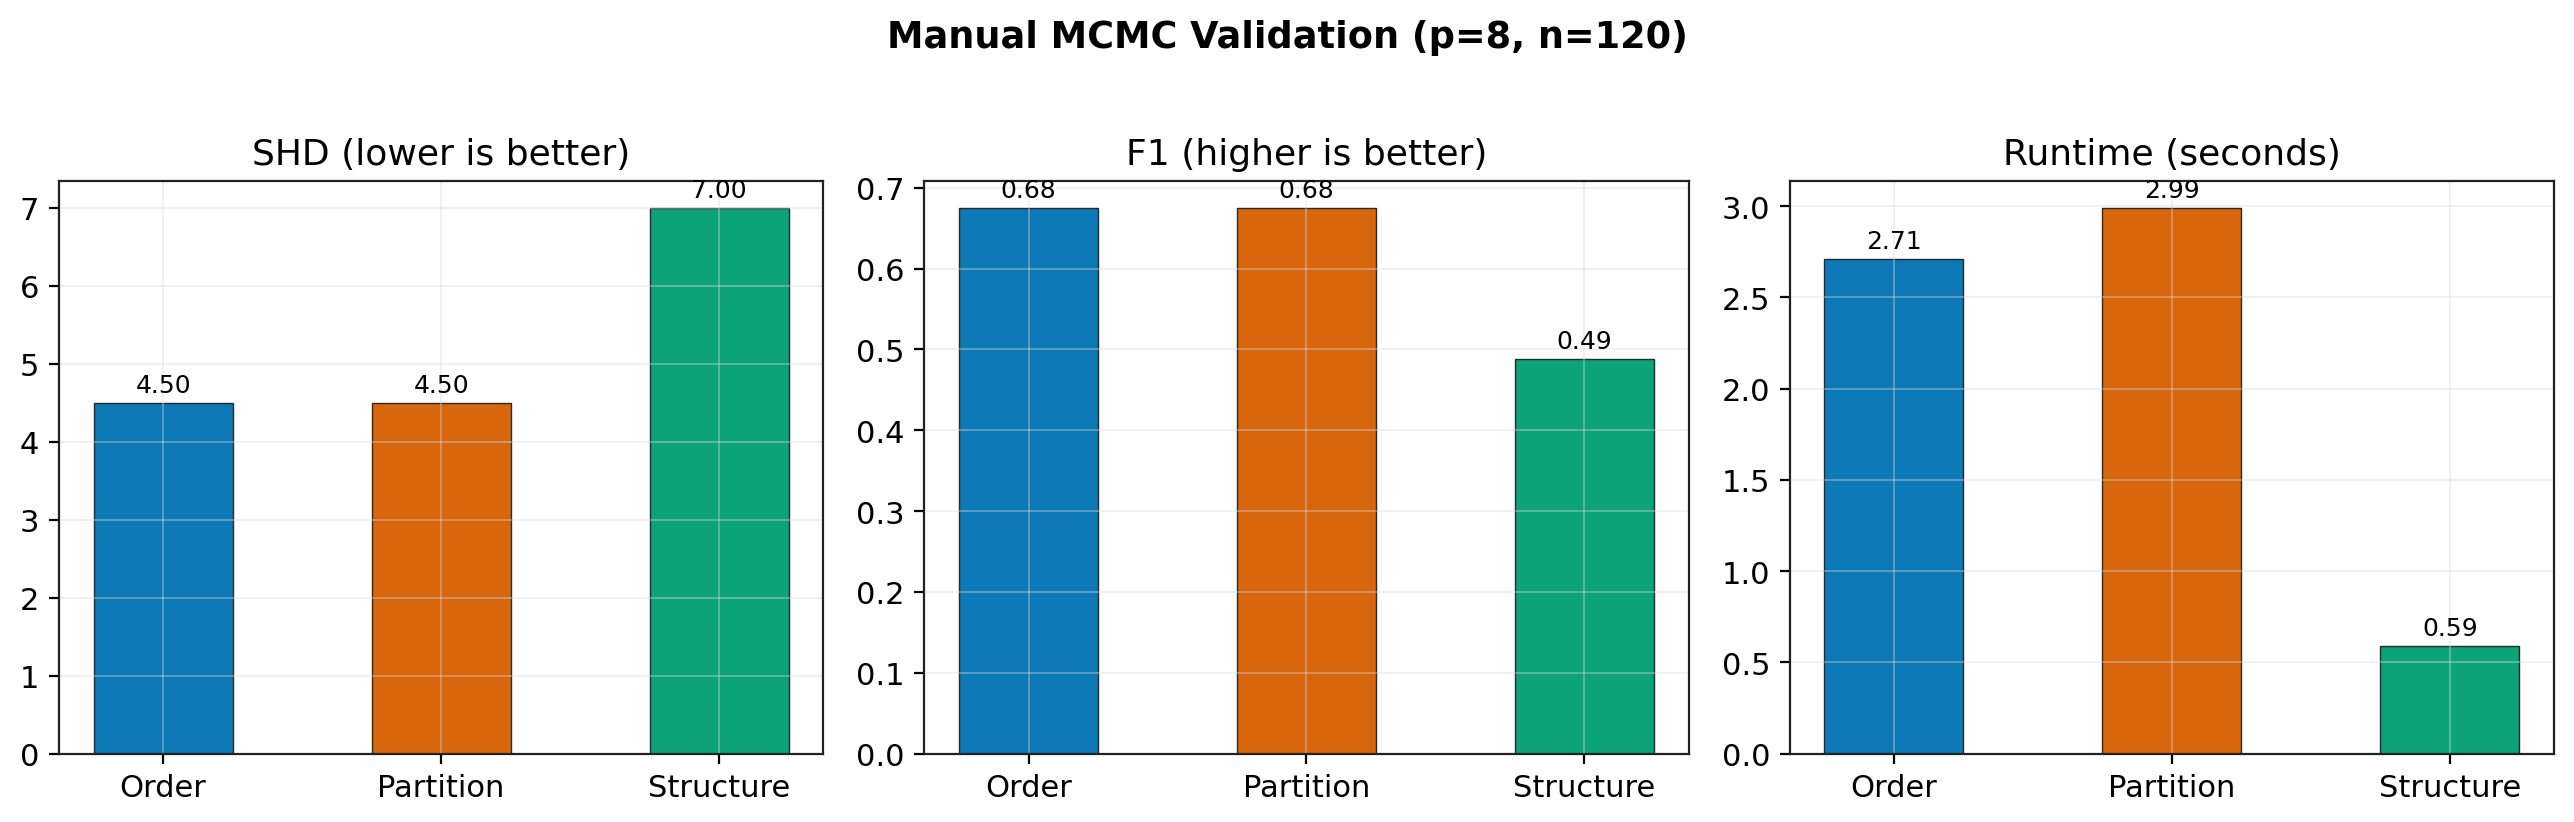
\includegraphics[width=0.88\linewidth]{py_manual_validation_combined.png}
\caption{自主 MCMC 三种方法的验证实验结果（$p=8, n=120$，2 个种子平均）}
\label{fig:manual}
\end{figure}

\begin{table}[H]
\centering
\small
\setlength{\tabcolsep}{2pt}
\caption{手工实现验证结果}
\label{tab:manual}
\begin{tabular}{lrrrrrr}
\toprule
方法 & 运行时间 & SHD & TPR & FPR & Precision & F1
\\
\midrule
manual\_order & 2.710 & 4.500 & 0.675 & 0.064 & 0.675 & 0.675 \\
manual\_partition & 2.990 & 4.500 & 0.675 & 0.064 & 0.675 & 0.675 \\
manual\_structure & 0.590 & 7.000 & 0.500 & 0.107 & 0.477 & 0.488 \\
\bottomrule
\end{tabular}
\end{table}

\begin{table}[H]
\centering
\small
\setlength{\tabcolsep}{2pt}
\caption{手工 MCMC 采样诊断摘要}
\label{tab:manual_diag}
\begin{tabular}{lrrrr}
\toprule
方法 & 接受率 & 最佳得分 & 平均边后验 & 后验熵
\\
\midrule
manual\_order & 0.351 & -1448.0 & 0.174 & 0.149 \\
manual\_partition & 0.459 & -1448.0 & 0.173 & 0.125 \\
manual\_structure & 0.436 & -1492.6 & 0.182 & 0.167 \\
\bottomrule
\end{tabular}
\end{table}


\subsection{自主实现与 BiDAG 的结果对比}

为避免将初步运行检查与正式实验混用，本节补充同参数对照实验。表 \ref{tab:manual_bidag_compare} 和图 \ref{fig:manual_bidag_compare} 均基于相同模拟设置：$p=8,n=120$，期望度为 2，随机种子为 1 和 2，每条链运行 1500 步并丢弃前 300 步 burn-in。自主实现显式比较父节点上限 $K=2$ 与 $K=3$；BiDAG 的 \texttt{sampleBN} 在本文调用方式下没有与自主实现完全对应的 $K$ 参数，因此表中记为 $K$ 不适用。二者仍存在评分函数差异：自主实现采用 Gaussian BIC 近似评分，BiDAG 采用 BGe 评分。

同参结果表明，默认 $K=2$ 时，manual\_order 的 SHD/F1 为 4.5/0.675，manual\_partition 为 5.5/0.575，均低于 BiDAG Order 的 2.5/0.743 和 BiDAG Partition 的 1.5/0.859。当 $K$ 提高到 3 后，manual\_order 与 manual\_partition 的 SHD/F1 均改善到 2.0/0.850，接近 BiDAG Partition 在该设置下的恢复精度。这表明自主实现的主要限制不完全来自状态空间思想本身，也与默认父集约束偏紧有关；当真实图中部分节点需要 3 个父节点时，$K=2$ 会限制可搜索模型空间。

效率差异也有明确来源，并且可以从 BiDAG 源码得到支持。BiDAG 的 CRAN GitHub 镜像\footnote{\url{https://github.com/cran/BiDAG}}在 \texttt{DESCRIPTION} 中说明：为了在较大 DAG 上实现有效推断，算法会根据数据剪枝搜索空间，先用 PC algorithm 得到 skeleton，再结合 search-and-score 进行迭代修正；同一源码还显示包导入并链接 \texttt{Rcpp}，\texttt{src/} 中包含通过 \texttt{.Call} 调用的 C++ 辅助函数，已安装包中也包含编译后的 \texttt{BiDAG.dll}。这些信息表明，BiDAG 的速度优势并非仅来自算法名称差异，而是搜索空间压缩、评分表复用和部分底层计算优化共同作用的结果。

与之相比，本文自主实现的定位是可审计的算法对照实现，而非经过底层优化的工程库。核心实现代码的预计算阶段显式枚举候选父集；Order 和 Partition 评分在每次 proposal 后重新按当前状态筛选允许父集并求和；DAG 输出阶段还需要反复构造邻接矩阵用于 MAP 图和边后验累积。这些步骤主要在解释型 R 层完成，包含循环、字符串键匹配和矩阵重新分配，常数开销高于包内封装实现。另一方面，$K$ 从 2 增至 3 会使每个节点的候选父集从 $\sum_{d=0}^{2}\binom{p-1}{d}$ 增至 $\sum_{d=0}^{3}\binom{p-1}{d}$，在 $p=8$ 时约从 29 个增至 64 个，局部评分查找和 proposal 评估成本同步上升。因此，自主实现 $K=3$ 虽然达到接近 BiDAG 的低维恢复精度，但运行时间仍更长：manual\_order 和 manual\_partition 分别约为 5.20 秒和 5.66 秒，而 BiDAG Order 与 Partition 分别约为 0.65 秒和 2.88 秒。综合来看，\textbf{自主实现提供了对评分、proposal 和 MH 接受机制的可解释对照；在以稳定性和运行效率为主要目标的结构学习任务中，BiDAG 等成熟实现更具工程优势。}

\begin{table}[htbp]
\centering
\small
\setlength{\tabcolsep}{4pt}
\caption{手工实现与 BiDAG 的同参数小规模对比（$p=8,n=120$，2 个种子平均，1500 步 MCMC，300 步 burn-in）}
\label{tab:manual_bidag_compare}
\begin{tabular}{lllrrrrrr}
\toprule
实现路径 & 方法 & 评分 / $K$ & 运行时间 & SHD & TPR & FPR & Precision & F1 \\
\midrule
BiDAG & Order & BGe, $K$ 不适用 & 0.650 & 2.500 & 0.725 & 0.043 & 0.764 & 0.743 \\
BiDAG & Partition & BGe, $K$ 不适用 & 2.875 & 1.500 & 0.838 & 0.021 & 0.882 & 0.859 \\
手工实现 & Structure & BIC, $K=2$ & 0.680 & 8.000 & 0.500 & 0.128 & 0.431 & 0.463 \\
手工实现 & Order & BIC, $K=2$ & 3.150 & 4.500 & 0.675 & 0.064 & 0.675 & 0.675 \\
手工实现 & Order & BIC, $K=3$ & 5.195 & 2.000 & 0.850 & 0.033 & 0.850 & 0.850 \\
手工实现 & Partition & BIC, $K=2$ & 3.360 & 5.500 & 0.575 & 0.086 & 0.575 & 0.575 \\
手工实现 & Partition & BIC, $K=3$ & 5.660 & 2.000 & 0.850 & 0.033 & 0.850 & 0.850 \\
\bottomrule
\end{tabular}
\end{table}


\begin{figure}[htbp]
\centering
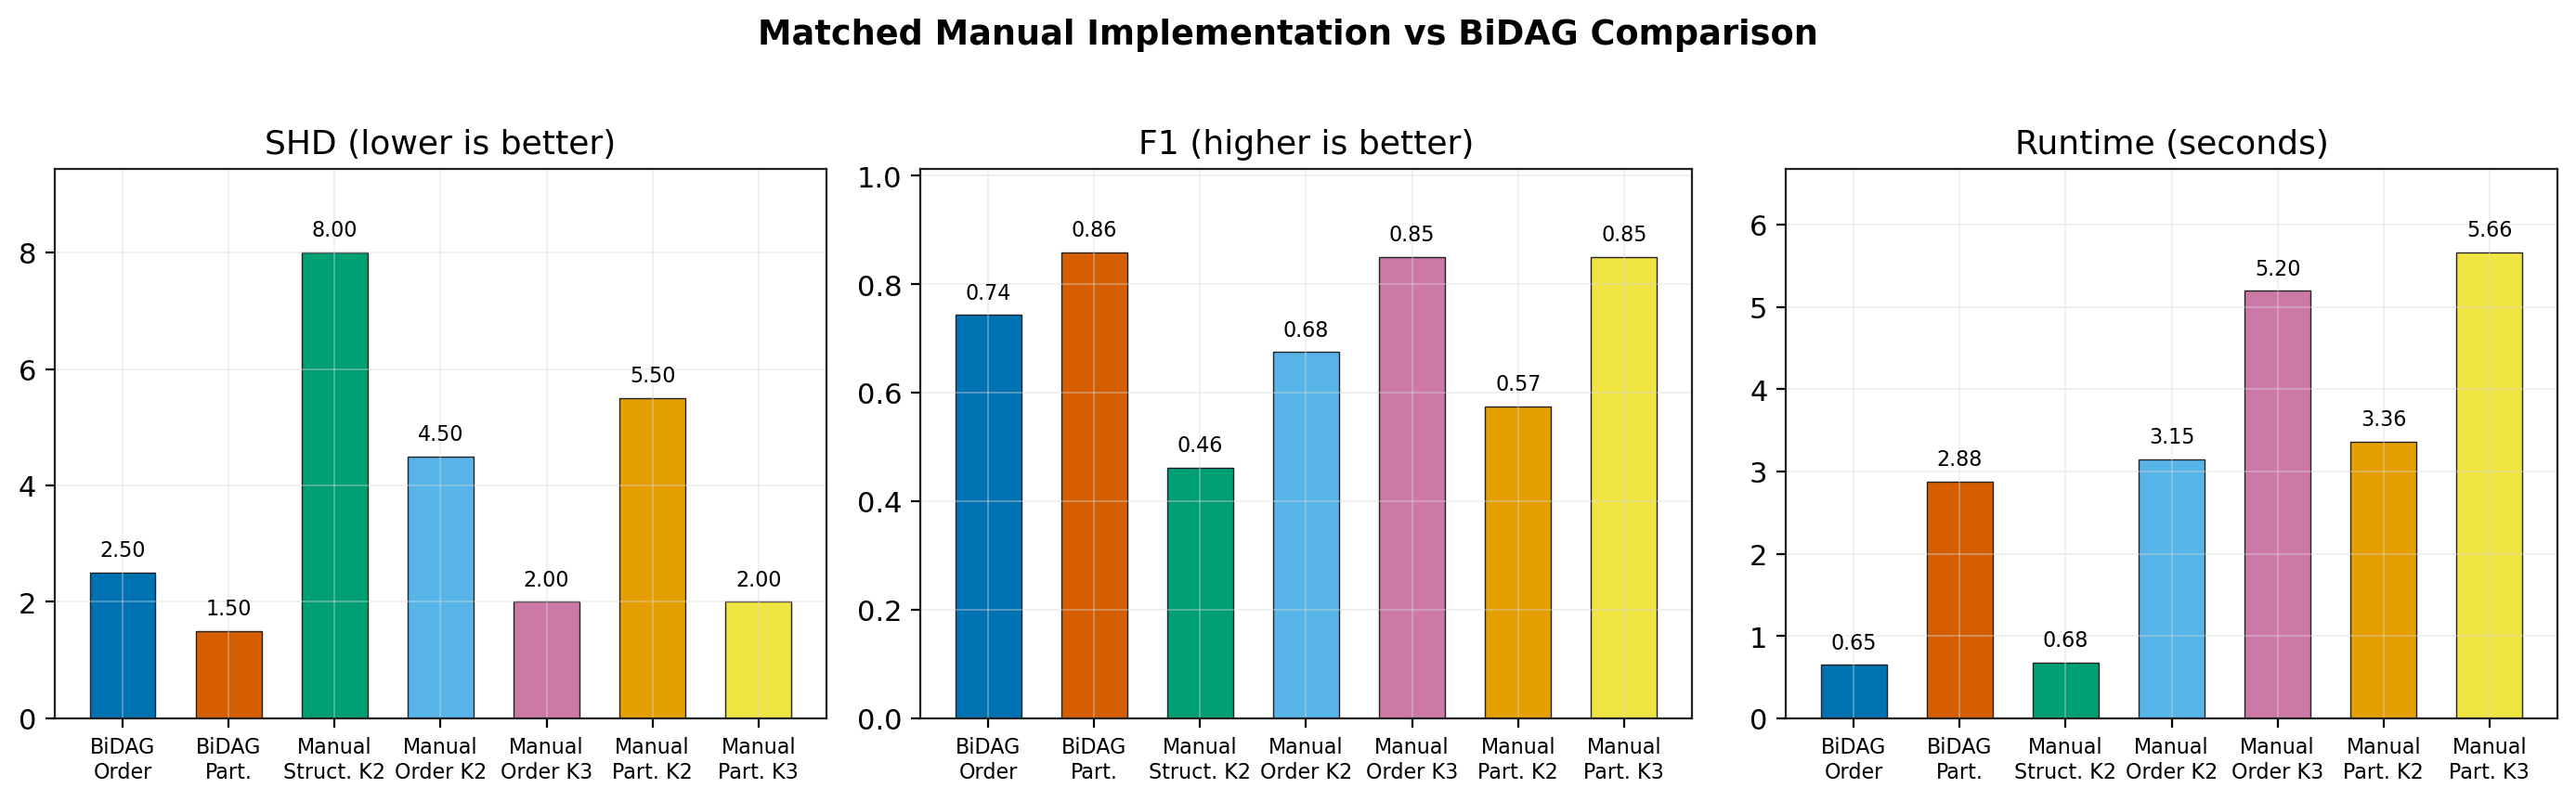
\includegraphics[width=0.92\linewidth]{py_manual_bidag_comparison.png}
\caption{自主实现与 BiDAG 的同参数对比（$p=8,n=120$，2 个种子平均）。自主实现方法显式设置父节点上限 $K$；BiDAG 行中的 $K$ 不适用}
\label{fig:manual_bidag_compare}
\end{figure}

\subsection{低维 Order 与 Partition 比较}

低维实验在 $p \in \{10, 20\}, n \in \{200, 500\}$ 的 12 个配置下比较 Order 和 Partition MCMC（3 个随机种子 $\times$ 4 个 $(p,n)$ 组合）。结果如表 \ref{tab:small} 所示。

结果：
\begin{enumerate}
  \item Partition MCMC 的运行时间约为 Order MCMC 的 3--5 倍。这一差距来自 partition 状态空间的组合权重计算和更复杂的 proposal 操作。
  \item 在 $p=10, n=500$ 的设置下，Partition MCMC 取得最低 SHD（1.67）和最高 F1（0.878），优于 Order MCMC 的 SHD=3.0, F1=0.789。
  \item 在 $p=20, n=200$ 时，Partition MCMC 表现低于 Order MCMC（SHD 5.67 vs 3.33）。这提示 Partition MCMC 的优势并非无条件的——在样本量相对不足时，其更复杂的状态空间可能带来额外的不确定性。
\end{enumerate}

这些观察说明：Partition MCMC 通过更精确的 DAG 表示降低了结构偏差，但需要较高样本量支持才能充分发挥这一优势。在样本量较小时，Order MCMC 较低的状态表示和 proposal 计算开销反而形成优势。

\begin{table}[H]
\centering
\small
\setlength{\tabcolsep}{2pt}
\caption{小规模 Order MCMC 与 Partition MCMC 比较}
\label{tab:small}
\begin{tabular}{lrrrrrrrr}
\toprule
方法 & p & n & 运行时间 & SHD & TPR & FPR & Precision & F1
\\
\midrule
order & 10.000 & 200.0 & 1.150 & 3.333 & 0.796 & 0.038 & 0.758 & 0.776 \\
partition & 10.000 & 200.0 & 5.027 & 3.000 & 0.787 & 0.038 & 0.746 & 0.766 \\
order & 20.000 & 200.0 & 1.427 & 3.333 & 0.851 & 0.008 & 0.831 & 0.841 \\
partition & 20.000 & 200.0 & 6.920 & 5.667 & 0.821 & 0.016 & 0.705 & 0.758 \\
order & 10.000 & 500.0 & 1.327 & 3.000 & 0.796 & 0.034 & 0.781 & 0.789 \\
partition & 10.000 & 500.0 & 5.450 & 1.667 & 0.889 & 0.021 & 0.868 & 0.878 \\
order & 20.000 & 500.0 & 1.667 & 3.000 & 0.860 & 0.007 & 0.841 & 0.850 \\
partition & 20.000 & 500.0 & 6.400 & 3.000 & 0.860 & 0.008 & 0.828 & 0.844 \\
\bottomrule
\end{tabular}
\end{table}


\begin{figure}[htbp]
\centering
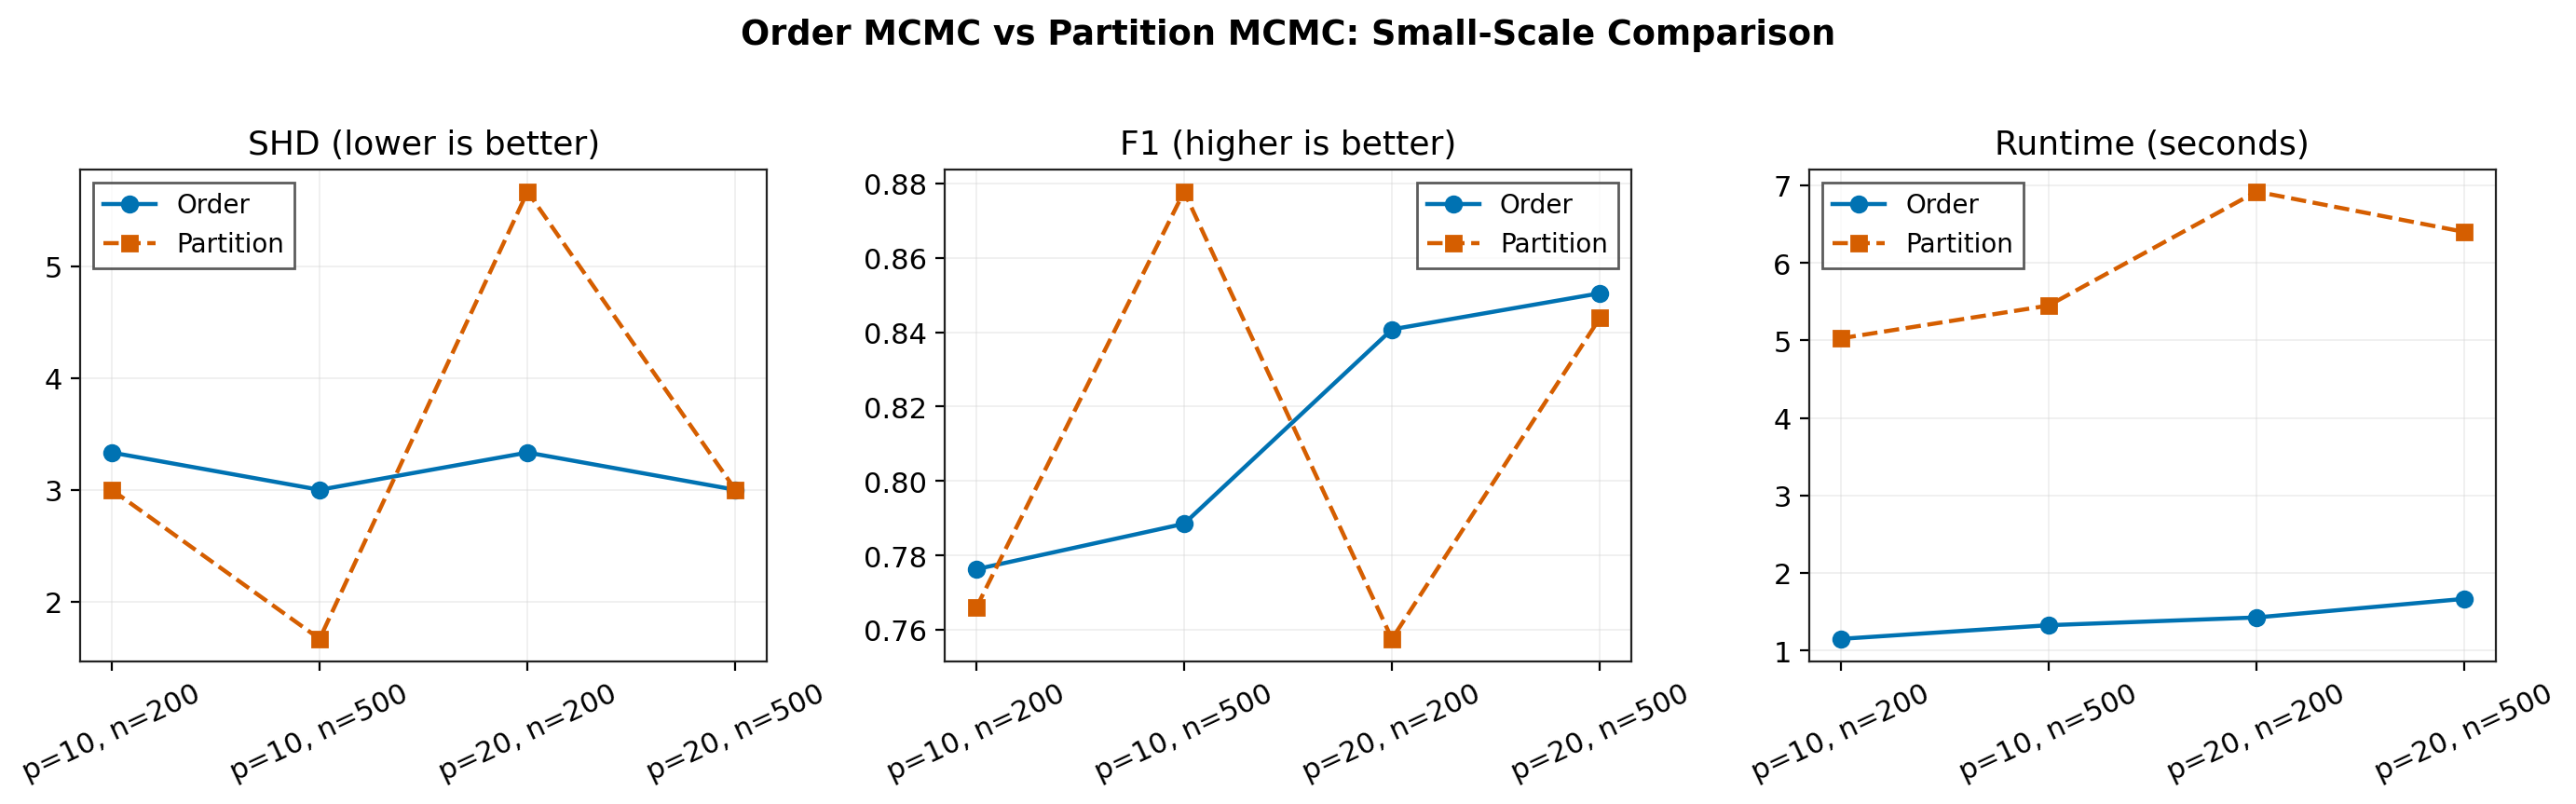
\includegraphics[width=0.88\linewidth]{py_small_compare_combined.png}
\caption{低维实验中 Order MCMC 与 Partition MCMC 的性能对比（$p \in \{10,20\}$, $n \in \{200,500\}$，3 个种子平均）}
\label{fig:small}
\end{figure}

\subsection{中等规模可扩展性}

中等规模实验采用 $p=30, n=500$ 设置。该规模已经能够体现节点数增加后普通 MCMC 方法面临的搜索压力，同时仍能保持多次重复实验的稳定完成，因而适合作为本文主线比较的一部分。

表 \ref{tab:medium} 显示，在 $p=30$ 下 Partition MCMC 的 SHD（5.0）低于 Order MCMC（14.0），F1（0.795 vs 0.672）也有一定优势。从 $p=20$ 到 $p=30$，Order MCMC 的 SHD 从约 3.3 增至 14.0，表明其在该维度附近的搜索效率出现下降。Partition MCMC 的退化幅度较小（从 3.0 至 5.0），在该设置下表现出较好的规模适应性。

这一对比也解释了 hybrid/iterative 策略的动机：当节点数继续增加时，普通 MCMC 的搜索压力会同步上升，通过预筛选缩小搜索空间有助于维持实用精度。

\begin{table}[H]
\centering
\small
\setlength{\tabcolsep}{2pt}
\caption{中等规模实验结果}
\label{tab:medium}
\begin{tabular}{lrrrrrrrr}
\toprule
方法 & p & n & 运行时间 & SHD & TPR & FPR & Precision & F1
\\
\midrule
order & 30.000 & 500.0 & 1.080 & 14.000 & 0.720 & 0.016 & 0.633 & 0.672 \\
partition & 30.000 & 500.0 & 2.875 & 5.000 & 0.802 & 0.006 & 0.789 & 0.795 \\
\bottomrule
\end{tabular}
\end{table}


\subsection{Iterative MCMC 规模扩展补充实验}

为观察预筛选与迭代修正策略在较大节点数下的表现，本文补充 $p=40,n=500$ 的 iterative MCMC 实验。该实验不作为大规模网络复现，而是用于说明在节点数增加时，约束候选边集合的搜索策略是否仍能给出可解释的结构恢复结果。

表 \ref{tab:highdim} 显示 iterative MCMC 在 $p=40$ 下完成两个种子的实验，seed 1 的 SHD 为 20（F1=0.515），seed 2 的 SHD 为 10（F1=0.870）。两个种子之间的差异较大，提示该类 MCMC 结果对随机初始化较为敏感，单次运行的 MAP 估计可能不够稳健。这一观察进一步支持了本文引入多链收敛诊断方案的必要性。

从方法机制看，hybrid/iterative 策略通过条件独立筛选压缩候选空间，使后续 MCMC 主要集中在较可能存在的边上。本文仅将该实验作为规模扩展的补充观察，不进一步展开更大规模网络设置。

\begin{table}[H]
\centering
\small
\setlength{\tabcolsep}{2pt}
\caption{Iterative MCMC 补充实验结果}
\label{tab:highdim}
\begin{tabular}{lrrrrrrrr}
\toprule
方法 & p & n & 运行时间 & SHD & TPR & FPR & Precision & F1
\\
\midrule
iterative & 40.000 & 500.0 & 13.720 & 15.000 & 0.745 & 0.010 & 0.649 & 0.693 \\
\bottomrule
\end{tabular}
\end{table}


\subsection{边后验不确定性分析}

基于实验原始输出中存储的成功运行结果，本文计算了第 4.2 节定义的三种不确定性指标。图 \ref{fig:posterior} 汇总了主要发现。

主要结果：

\begin{enumerate}
  \item \textbf{Partition MCMC 在多数可比设置下给出了与 Order MCMC 接近或更低的边后验熵，尤其在中等规模设置中差异更清晰。} 例如在 $p=20,n=500$ 下，Order MCMC 的 entropy 为 0.057，Partition MCMC 为 0.058，二者几乎相同；而在 $p=30,n=500$ 下，Order MCMC 为 0.056，Partition MCMC 为 0.029，Partition 的结构不确定性较低。该结果提示，partition 表示在部分中等规模设置下可能有助于减少结构模糊性，但这一结论仍受样本量、随机种子和链长影响。

  \item \textbf{高不确定性边的比例随 $p$ 增大而下降。} 其原因并非节点数增加后方法必然更"确定"，而是候选边数量以 $O(p^2)$ 增长，而真实边的期望数量仅以 $O(p \cdot d)$ 增长——这意味着绝大多数边对的真实状态为"不存在"，而后验概率容易集中在 0 附近。

  \item \textbf{Iterative MCMC 在 $p=40$ 下仍然保持了合理的后验分离度。} 其 true edge mean posterior（0.776）远高于 false edge mean posterior（0.013），表明在缩小后的搜索空间中，方法仍能有效区分信号和噪声。

  \item \textbf{True/False posterior gap 随样本量增大而改善。} 在 $n$ 从 100 增至 1000 的过程中，Order 和 Partition 的 posterior gap 均单调增大，说明更多数据有助于方法更清晰地区分真实边和虚假边。
\end{enumerate}

图 \ref{fig:posterior} 从两个维度可视化了上述发现：图 \ref{fig:posterior}(a) 给出不同 $(p,n)$ 组合下各方法的平均边后验熵，图 \ref{fig:posterior}(b) 给出真假边后验概率的分离度随样本量的变化趋势。

\begin{figure}[htbp]
\centering
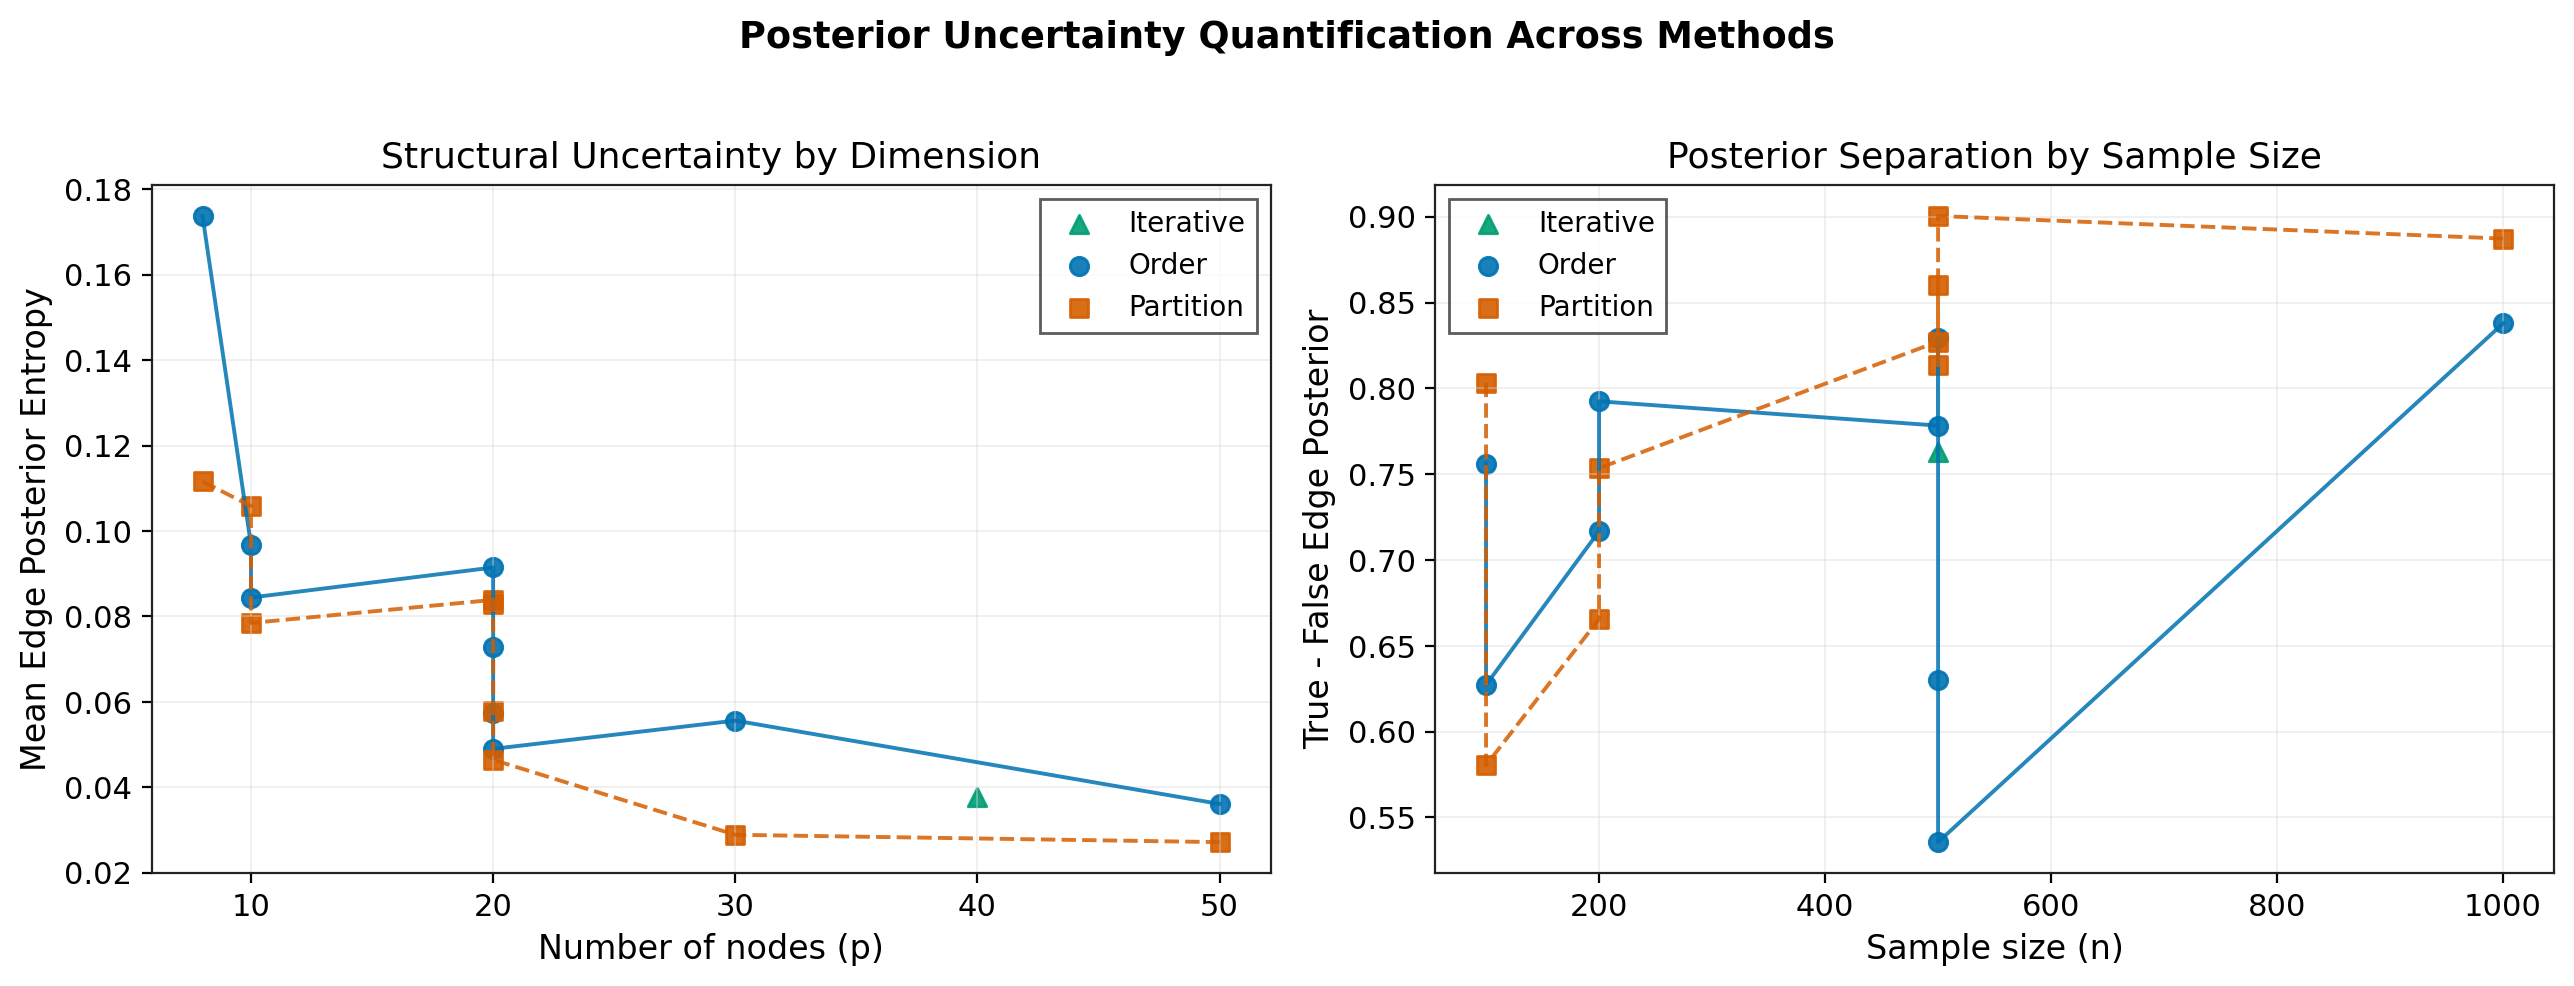
\includegraphics[width=0.88\linewidth]{py_posterior_uncertainty_combined.png}
\caption{边后验不确定性分析。左：平均边后验熵随维度 $p$ 的变化；右：真边与假边后验概率的分离度随样本量 $n$ 的变化}
\label{fig:posterior}
\end{figure}

\subsection{样本量影响}

样本量实验固定 $p=20$，在 $n \in \{100, 200, 500, 1000\}$ 四个水平下比较 Order 和 Partition MCMC。表 \ref{tab:sample} 显示：

\begin{enumerate}
  \item 随着样本量增大，Order MCMC 的 SHD 从 8.0（$n=100$）单调下降至 2.67（$n=1000$），F1 从 0.728 上升至 0.868。这与统计估计的一般规律一致：更多数据提供更准确的局部回归评分，从而改善父集选择。

  \item Partition MCMC 在 $n=100$ 时表现较弱（SHD=9.0, F1=0.598），但在 $n=500$ 和 $n=1000$ 时接近（SHD 均为 3.0 和 2.67）。这表明 Partition MCMC 需要较高样本量来克服其更复杂的状态空间带来的额外自由度。

  \item 运行时间随 $n$ 的变化幅度较小，说明计算瓶颈主要在 MCMC 迭代次数和 $p$，而非样本量本身。这是因为 BiDAG 的评分函数在给定数据后，局部评分计算是一次性完成的，MCMC 迭代过程中只需查表。
\end{enumerate}

\begin{figure}[htbp]
\centering
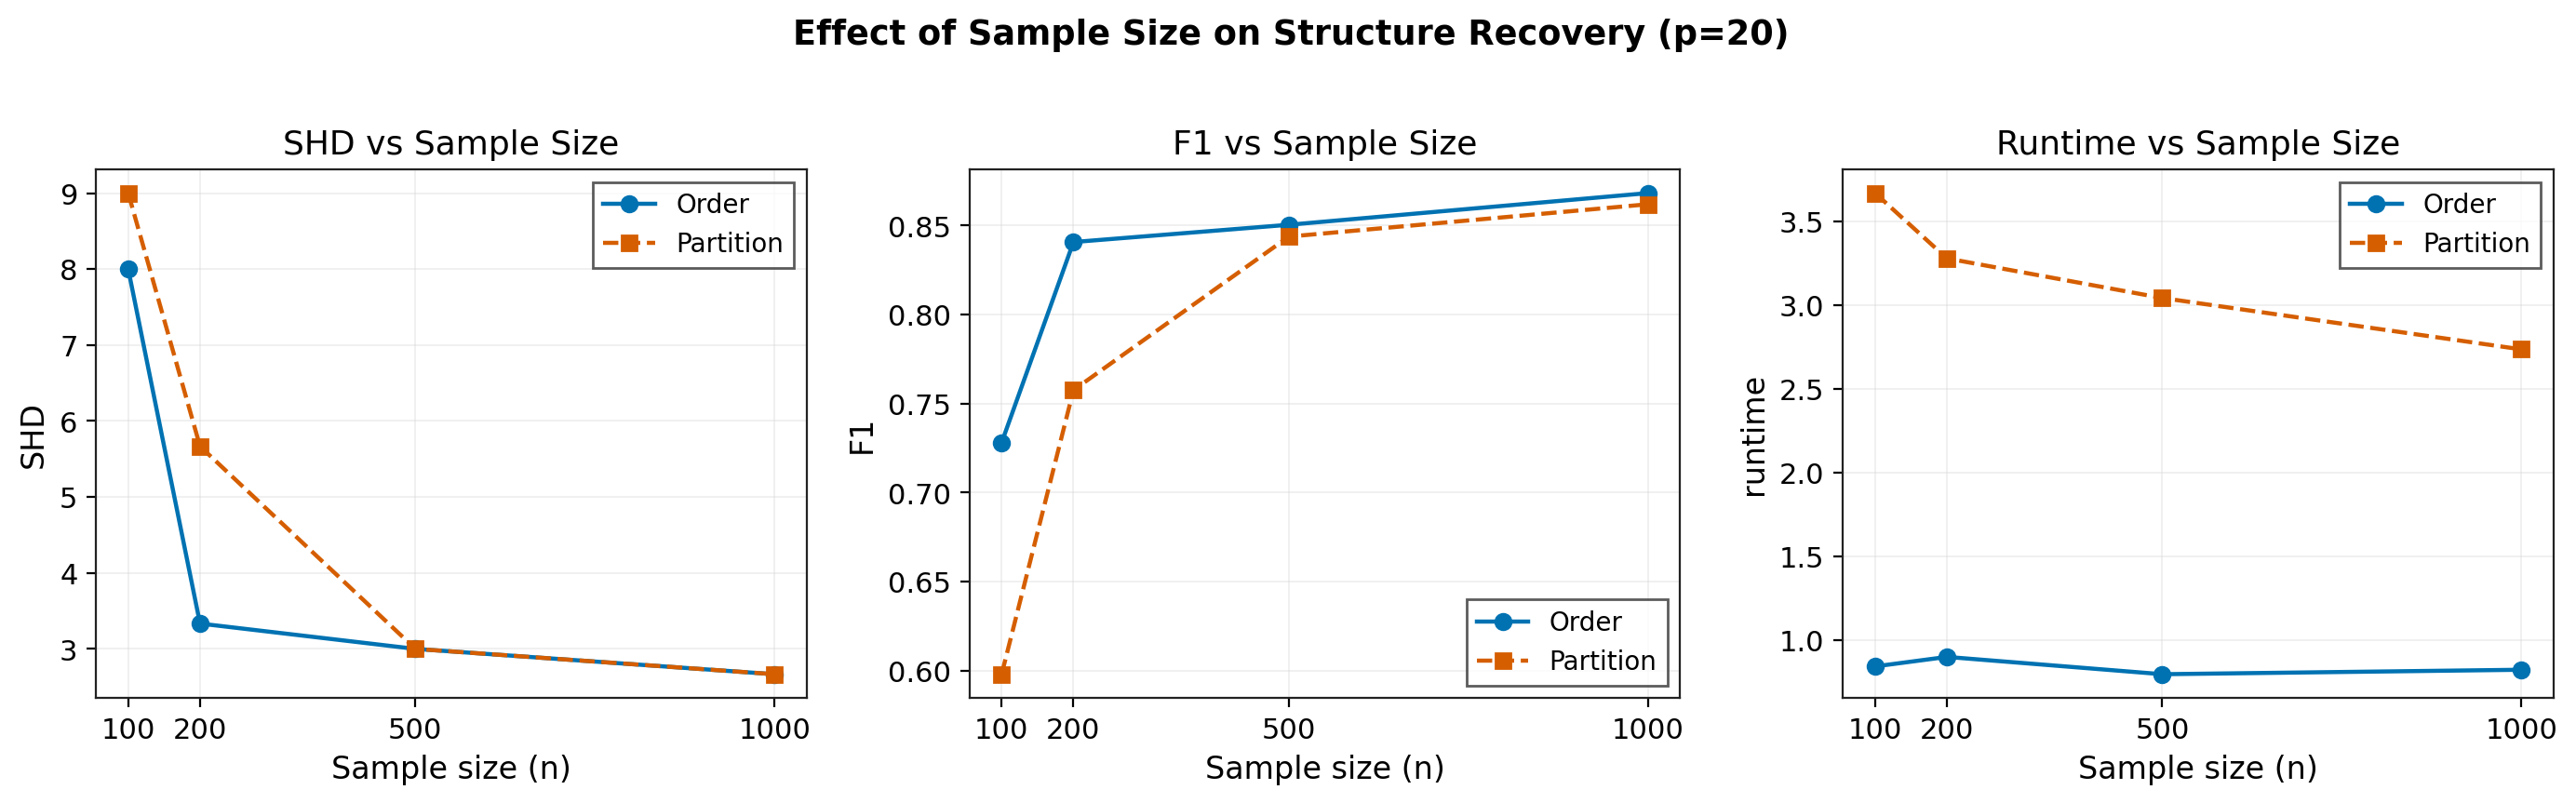
\includegraphics[width=0.88\linewidth]{py_sample_size_combined.png}
\caption{样本量对 Order MCMC 与 Partition MCMC 结构恢复精度的影响（$p=20$, $n \in \{100,200,500,1000\}$，3 个种子平均）}
\label{fig:sample}
\end{figure}

\begin{table}[H]
\centering
\small
\setlength{\tabcolsep}{2pt}
\caption{样本量影响实验结果}
\label{tab:sample}
\begin{tabular}{lrrrrrrrr}
\toprule
方法 & p & n & 运行时间 & SHD & TPR & FPR & Precision & F1
\\
\midrule
order & 20.000 & 100.0 & 0.843 & 8.000 & 0.768 & 0.016 & 0.694 & 0.728 \\
partition & 20.000 & 100.0 & 3.670 & 9.000 & 0.640 & 0.023 & 0.562 & 0.598 \\
order & 20.000 & 200.0 & 0.900 & 3.333 & 0.851 & 0.008 & 0.831 & 0.841 \\
partition & 20.000 & 200.0 & 3.280 & 5.667 & 0.821 & 0.016 & 0.705 & 0.758 \\
order & 20.000 & 500.0 & 0.797 & 3.000 & 0.860 & 0.007 & 0.841 & 0.850 \\
partition & 20.000 & 500.0 & 3.043 & 3.000 & 0.860 & 0.008 & 0.828 & 0.844 \\
order & 20.000 & 1000.0 & 0.823 & 2.667 & 0.868 & 0.006 & 0.868 & 0.868 \\
partition & 20.000 & 1000.0 & 2.737 & 2.667 & 0.868 & 0.007 & 0.856 & 0.862 \\
\bottomrule
\end{tabular}
\end{table}


\subsection{父节点集约束敏感性}

父集约束敏感性实验在 $p=8, n=120$ 下比较 $K \in \{1, 2, 3\}$ 三种设置对三种自主实现方法的影响。表 \ref{tab:manual_sensitivity} 的关键发现：

\begin{enumerate}
  \item 当 $K=1$ 时，所有方法的表现均较差（F1 在 0.19--0.45 之间），因为 $K=1$ 不足以捕获真实图中可能需要多个父节点的依赖关系。

  \item 从 $K=2$ 到 $K=3$，manual\_order 和 manual\_partition 的 F1 从 0.675 增至 0.85，SHD 从 4.5 降至 2.0。这表明父集容量增加后结构恢复有所改善。运行时间从约 4.6 秒增至约 7.5 秒，计算代价仍处于可接受范围。

  \item manual\_structure 在所有 $K$ 设置下均弱于另外两种方法，只在 $K=3$ 时 F1 达到 0.556。即使在放宽的父集约束下，直接 DAG 空间搜索的困难仍然存在。
\end{enumerate}

这些结果支持了第 4.1 节自适应父集策略的动机：不同节点和不同网络密度可能需要不同的 $K$ 值，固定约束的精度--效率权衡可以通过自适应调整来改善。

\begin{table}[H]
\centering
\small
\setlength{\tabcolsep}{2pt}
\caption{手工 MCMC 最大父节点数敏感性实验}
\label{tab:manual_sensitivity}
\begin{tabular}{lrrrrrr}
\toprule
方法 & 最大父节点数 & 运行时间 & SHD & Precision & Recall & F1
\\
\midrule
manual\_order & 1.000 & 1.955 & 6.000 & 0.452 & 0.325 & 0.378 \\
manual\_partition & 1.000 & 2.790 & 5.500 & 0.536 & 0.388 & 0.450 \\
manual\_structure & 1.000 & 0.680 & 10.500 & 0.226 & 0.163 & 0.189 \\
manual\_order & 2.000 & 4.625 & 4.500 & 0.675 & 0.675 & 0.675 \\
manual\_partition & 2.000 & 4.965 & 5.500 & 0.575 & 0.575 & 0.575 \\
manual\_structure & 2.000 & 0.890 & 8.000 & 0.431 & 0.500 & 0.463 \\
manual\_order & 3.000 & 7.545 & 2.000 & 0.850 & 0.850 & 0.850 \\
manual\_partition & 3.000 & 7.845 & 2.000 & 0.850 & 0.850 & 0.850 \\
manual\_structure & 3.000 & 0.905 & 6.500 & 0.518 & 0.600 & 0.556 \\
\bottomrule
\end{tabular}
\end{table}


\begin{figure}[htbp]
\centering
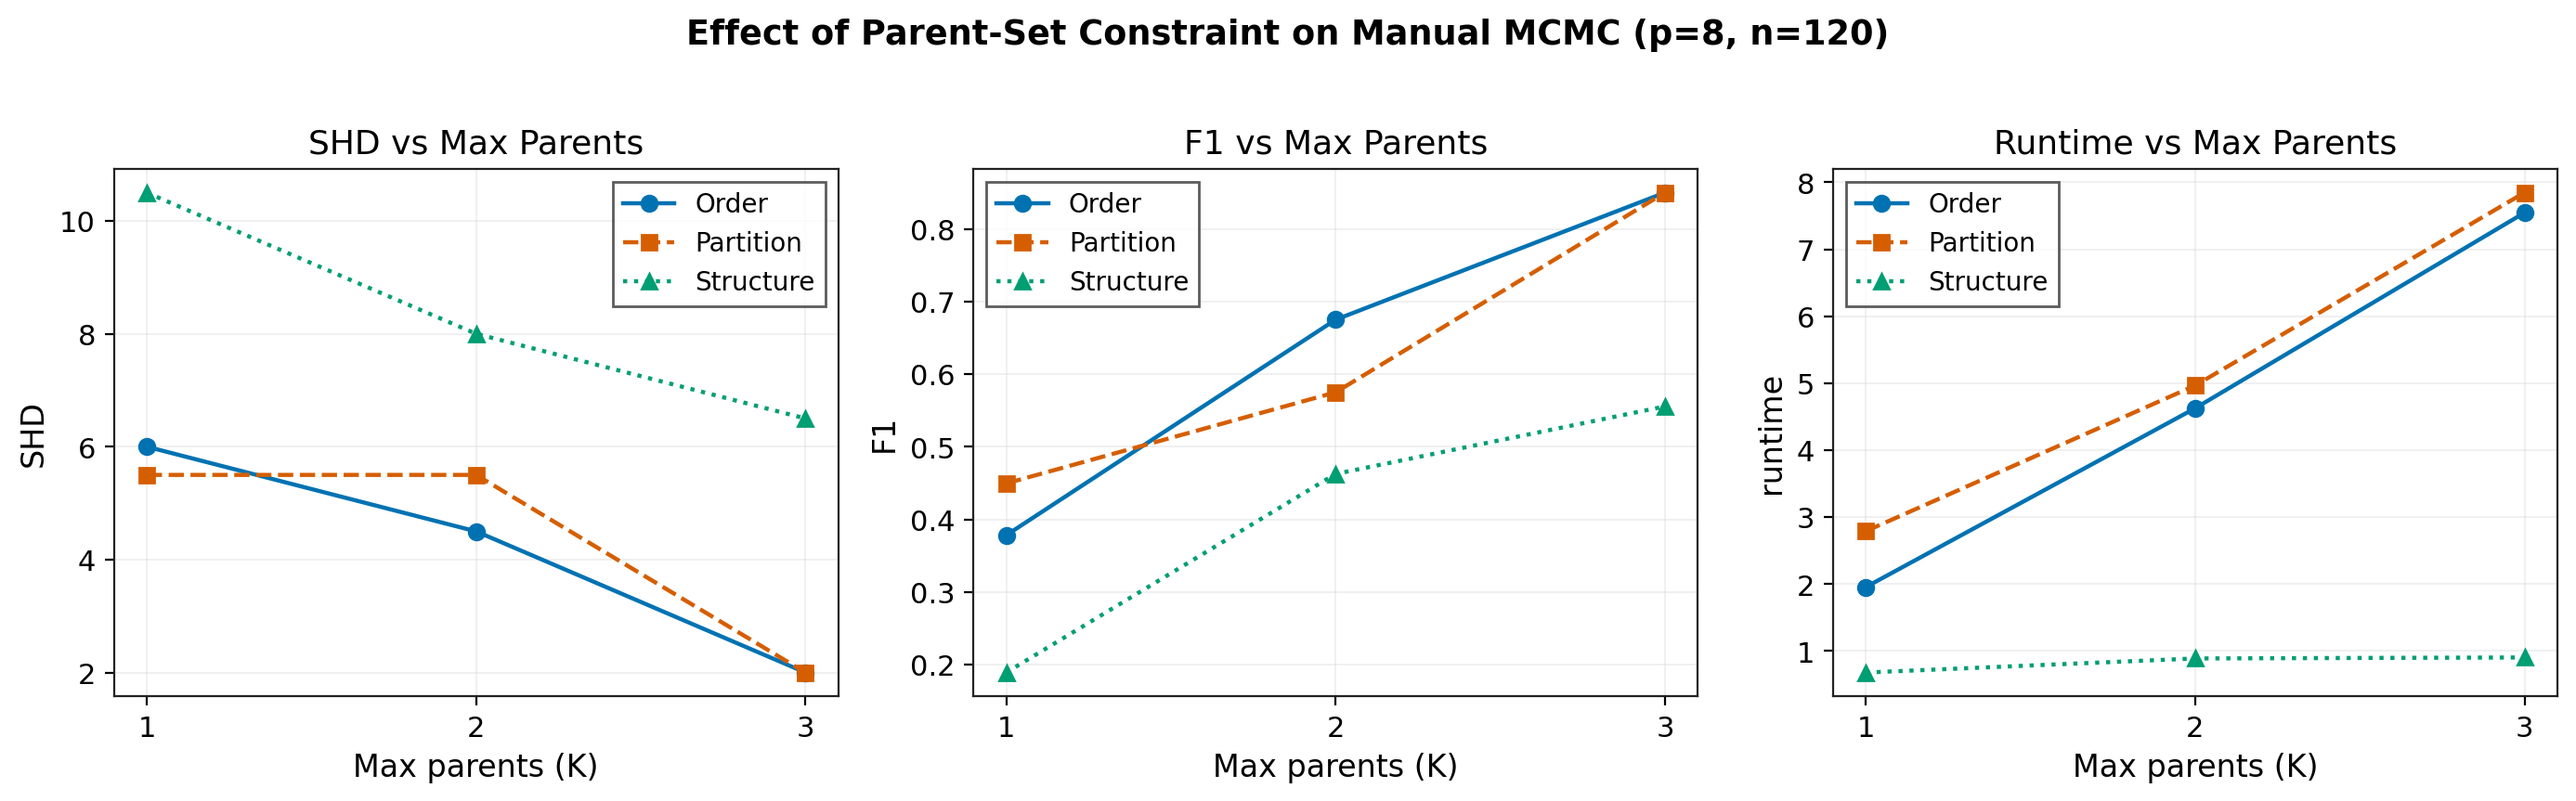
\includegraphics[width=0.88\linewidth]{py_manual_sensitivity_combined.png}
\caption{父节点集上限 $K$ 对三种自主 MCMC 方法性能的影响（$p=8, n=120$，2 个种子平均）}
\label{fig:sensitivity}
\end{figure}

\FloatBarrier
\newpage

\subsection{中等规模关键论文趋势对照实验}

为进一步说明本文实验与原始文献的关系，并比较不同实现路径在中等规模设置下的精度与效率差异，本文补充中等规模原论文对照复现实验。该实验包含三类实现：纯 Python/numpy 实现、R 自主实现和 BiDAG 官方包实现。其中 Python 与 R 自主实现均采用 Gaussian BIC 型评分，主要用于交叉检查自主算法逻辑；BiDAG 采用其包内 BGe 评分和底层优化实现，作为成熟软件基准。所有数据均为模拟生成（分别标记为 simulated\_flare\_like、simulated\_alarm\_like、simulated\_toy\_like、simulated\_boston\_like 和 simulated\_large\_like），未使用真实 ALARM 或 Boston Housing 数据。实验共生成 20 组模拟数据，三类实现共完成 134 次 MCMC 采样。

\begin{table}[htbp]
\centering\footnotesize
\caption{中等规模原论文对照实验结果（按维度 $p$ 和方法聚合，平均所有 $n$)}
\label{tab:medium_original_summary}
\setlength{\tabcolsep}{3pt}
\begin{tabular}{c c l l c c c c}
\toprule
$p$ & Experiment & Method & Impl & Mean SHD & F1 & TPR & Time(s) \\
\midrule
5 & Partition MCMC (K\&M 2017) & manual\_order & mR & 2.2 & 0.646 & 0.700 & 0.7 \\
5 & Partition MCMC (K\&M 2017) & manual\_partition & mR & 2.2 & 0.646 & 0.700 & 0.9 \\
5 & Partition MCMC (K\&M 2017) & manual\_structure & mR & 2.2 & 0.655 & 0.700 & 0.4 \\
5 & Partition MCMC (K\&M 2017) & order & BD & 0.0 & 1.000 & 1.000 & 0.5 \\
5 & Partition MCMC (K\&M 2017) & partition & BD & 0.0 & 1.000 & 1.000 & 1.5 \\
5 & Partition MCMC (K\&M 2017) & python\_order & Py & 1.8 & 0.737 & 0.800 & 0.0 \\
5 & Partition MCMC (K\&M 2017) & python\_structure & Py & 4.8 & 0.379 & 0.483 & 0.0 \\
\addlinespace[2pt]
9 & Order MCMC (F\&K 2003) & manual\_order & mR & 5.8 & 0.601 & 0.620 & 2.5 \\
9 & Order MCMC (F\&K 2003) & manual\_partition & mR & 6.5 & 0.560 & 0.582 & 2.7 \\
9 & Order MCMC (F\&K 2003) & manual\_structure & mR & 12.2 & 0.358 & 0.389 & 0.4 \\
9 & Order MCMC (F\&K 2003) & order & BD & 3.2 & 0.799 & 0.791 & 0.6 \\
9 & Order MCMC (F\&K 2003) & partition & BD & 2.0 & 0.817 & 0.817 & 3.0 \\
9 & Order MCMC (F\&K 2003) & python\_order & Py & 5.8 & 0.601 & 0.620 & 0.0 \\
9 & Order MCMC (F\&K 2003) & python\_structure & Py & 12.5 & 0.366 & 0.435 & 0.0 \\
\addlinespace[2pt]
14 & Partition MCMC (K\&M 2017) & manual\_order & mR & 7.8 & 0.604 & 0.629 & 6.8 \\
14 & Partition MCMC (K\&M 2017) & manual\_partition & mR & 8.2 & 0.606 & 0.632 & 7.3 \\
14 & Partition MCMC (K\&M 2017) & manual\_structure & mR & 13.5 & 0.449 & 0.462 & 0.5 \\
14 & Partition MCMC (K\&M 2017) & order & BD & 3.0 & 0.835 & 0.842 & 0.9 \\
14 & Partition MCMC (K\&M 2017) & partition & BD & 4.2 & 0.773 & 0.779 & 4.5 \\
14 & Partition MCMC (K\&M 2017) & python\_order & Py & 7.2 & 0.639 & 0.665 & 0.1 \\
14 & Partition MCMC (K\&M 2017) & python\_structure & Py & 19.5 & 0.376 & 0.444 & 0.1 \\
\addlinespace[2pt]
20 & Partition MCMC (K\&M 2017) & manual\_order & mR & 11.0 & 0.635 & 0.628 & 21.9 \\
20 & Partition MCMC (K\&M 2017) & manual\_partition & mR & 16.0 & 0.526 & 0.539 & 20.0 \\
20 & Partition MCMC (K\&M 2017) & manual\_structure & mR & 33.5 & 0.253 & 0.266 & 1.0 \\
20 & Partition MCMC (K\&M 2017) & order & BD & 10.2 & 0.677 & 0.673 & 0.7 \\
20 & Partition MCMC (K\&M 2017) & partition & BD & 5.0 & 0.832 & 0.840 & 4.9 \\
20 & Partition MCMC (K\&M 2017) & python\_order & Py & 10.5 & 0.651 & 0.639 & 0.3 \\
20 & Partition MCMC (K\&M 2017) & python\_structure & Py & 39.0 & 0.183 & 0.204 & 0.3 \\
\addlinespace[2pt]
37 & Order MCMC (F\&K 2003) & manual\_order & mR & 24.8 & 0.604 & 0.672 & 118.1 \\
37 & Order MCMC (F\&K 2003) & manual\_structure & mR & 56.2 & 0.199 & 0.177 & 2.4 \\
37 & Order MCMC (F\&K 2003) & order & BD & 18.0 & 0.699 & 0.761 & 1.3 \\
37 & Order MCMC (F\&K 2003) & python\_order & Py & 21.2 & 0.645 & 0.701 & 2.4 \\
37 & Order MCMC (F\&K 2003) & python\_structure & Py & 73.5 & 0.110 & 0.115 & 1.4 \\
\addlinespace[2pt]
40 & Hybrid/Iter (KSM 2022) & iterative & BD & 15.0 & 0.782 & 0.877 & 35.0 \\
\bottomrule
\end{tabular}
\begin{flushleft}\footnotesize Py = Python implementation, BD = BiDAG, mR = manual R. SHD/F1/TPR/Time averaged over all $n$ and seeds.\end{flushleft}
\end{table}


表 \ref{tab:medium_original_summary} 按实验组、维度 $p$、方法和实现方式汇总了全部结果。主要观察如下：

\begin{enumerate}
  \item \textbf{三类实现形成了精度--效率对照。} BiDAG 在多数可比设置下取得较好的结构恢复结果：$p=5$ 时 SHD 为 0，$p=9$ 时 partition 和 order 的 SHD 分别为 1.0 和 3.2，$p=20$ 时 partition 和 order 的 SHD 分别为 5.0 和 10.2，$p=37$ 时 order 的 SHD 为 18.0。Python 实现和 R 自主实现在 order MCMC 上给出了接近的恢复精度（例如 $p=37$ 时 Python order 的平均 SHD 为 21.2，manual\_order 为 24.8），说明两套自主代码在相同 BIC 评分框架下呈现出一致的趋势。BiDAG 结果通常更优，但这一差异同时受到评分函数、搜索空间处理和底层实现优化的影响，不能简单归因于单一因素。

  \item \textbf{Order MCMC 相比 Structure MCMC 具有更稳定的恢复表现。}
  \begin{table}[htbp]
\centering
\caption{Order MCMC 与 Structure MCMC 的性能差距随维度增大加速扩大（Python 实现，平均所有 $n$）}
\label{tab:order_vs_structure}
\begin{tabular}{c c c c c c c}
\toprule
$p$ & Data source & Order SHD & Order F1 & Struct SHD & Struct F1 & $\Delta$SHD \\
\midrule
5 & toy-like & 1.8 & 0.737 & 4.8 & 0.379 & +3 \\
9 & flare-like & 5.8 & 0.601 & 12.5 & 0.366 & +7 \\
14 & boston-like & 7.2 & 0.639 & 19.5 & 0.376 & +12 \\
20 & large-like & 10.5 & 0.651 & 39.0 & 0.183 & +28 \\
37 & alarm-like & 21.2 & 0.645 & 73.5 & 0.110 & +52 \\
\bottomrule
\end{tabular}
\end{table}

  表 \ref{tab:order_vs_structure} 给出了 Python 实现上两种方法在不同 $p$ 下的平均 SHD 和 F1 对比。$p=5$ 时 Structure MCMC 的 SHD 比 Order 高 3 个点；$p=20$ 时差距扩大至 28.5 个点；$p=37$ 时 Structure MCMC 的 SHD 达到 73.5、F1 降至 0.110。该趋势支持了 Friedman and Koller (2003) 关于状态空间重构的分析：直接在 DAG 空间中进行局部边操作时，维度增加会加重混合困难；Order MCMC 通过排列空间消除无环检查，在该组模拟实验中表现出更稳定的恢复效果。

  \item \textbf{Partition MCMC 在部分中等规模设置下表现较好。} BiDAG 实现的 partition MCMC 在 $p=20$ 时取得 SHD=5.0、F1=0.832，优于同条件下 BiDAG order 的 SHD=10.2、F1=0.677。该结果与 Kuipers and Moffa (2017) 关于 partition 表示可缓解排序偏差的观点相一致。需要注意的是，R 自主实现中的简化 partition（manual\_partition）在 $p=20$ 时仅取得 SHD=16.0、F1=0.526，与 BiDAG partition 仍有差距。这说明本文的对照实现不能等同于完整 Partition MCMC；完整算法还依赖 DAG 到 partition 的组合计数权重、更复杂的 proposal 机制以及包内 C++ 底层实现。

  \item \textbf{运行效率主要受实现方式影响。} Python/numpy 实现在多数维度下运行较快：$p=37$ 时 order MCMC 约需 2.4 秒，而 R 自主实现约需 118.1 秒。BiDAG 的 order 在 $p=37$ 下约需 1.3 秒，反映了其底层实现、评分表复用和搜索空间处理的综合优势。这一对比说明，R 自主实现的主要开销来自解释型 R 层的循环、矩阵操作和字符串键匹配；将核心评分和 proposal 逻辑迁移到 numpy 向量化或 C++ 后端预计可以降低运行时间。

  \item \textbf{Hybrid/iterative MCMC 在较大节点数设置下给出了补充参照。} BiDAG 的 iterative MCMC 在 $p=40, n=200$ 设置下完成 2 次独立运行，平均 SHD=15.0、F1=0.782，单次运行约 35 秒。与普通 Order MCMC 在 $p=37$ 下的结果相比，iterative 策略通过条件独立筛选缩小候选边集，在相近维度下取得了可比较的恢复精度。该结果与 Kuipers, Suter and Moffa (2022) 关于预筛选有助于控制候选空间规模的观点相一致。
\end{enumerate}

\begin{figure}[htbp]
\centering
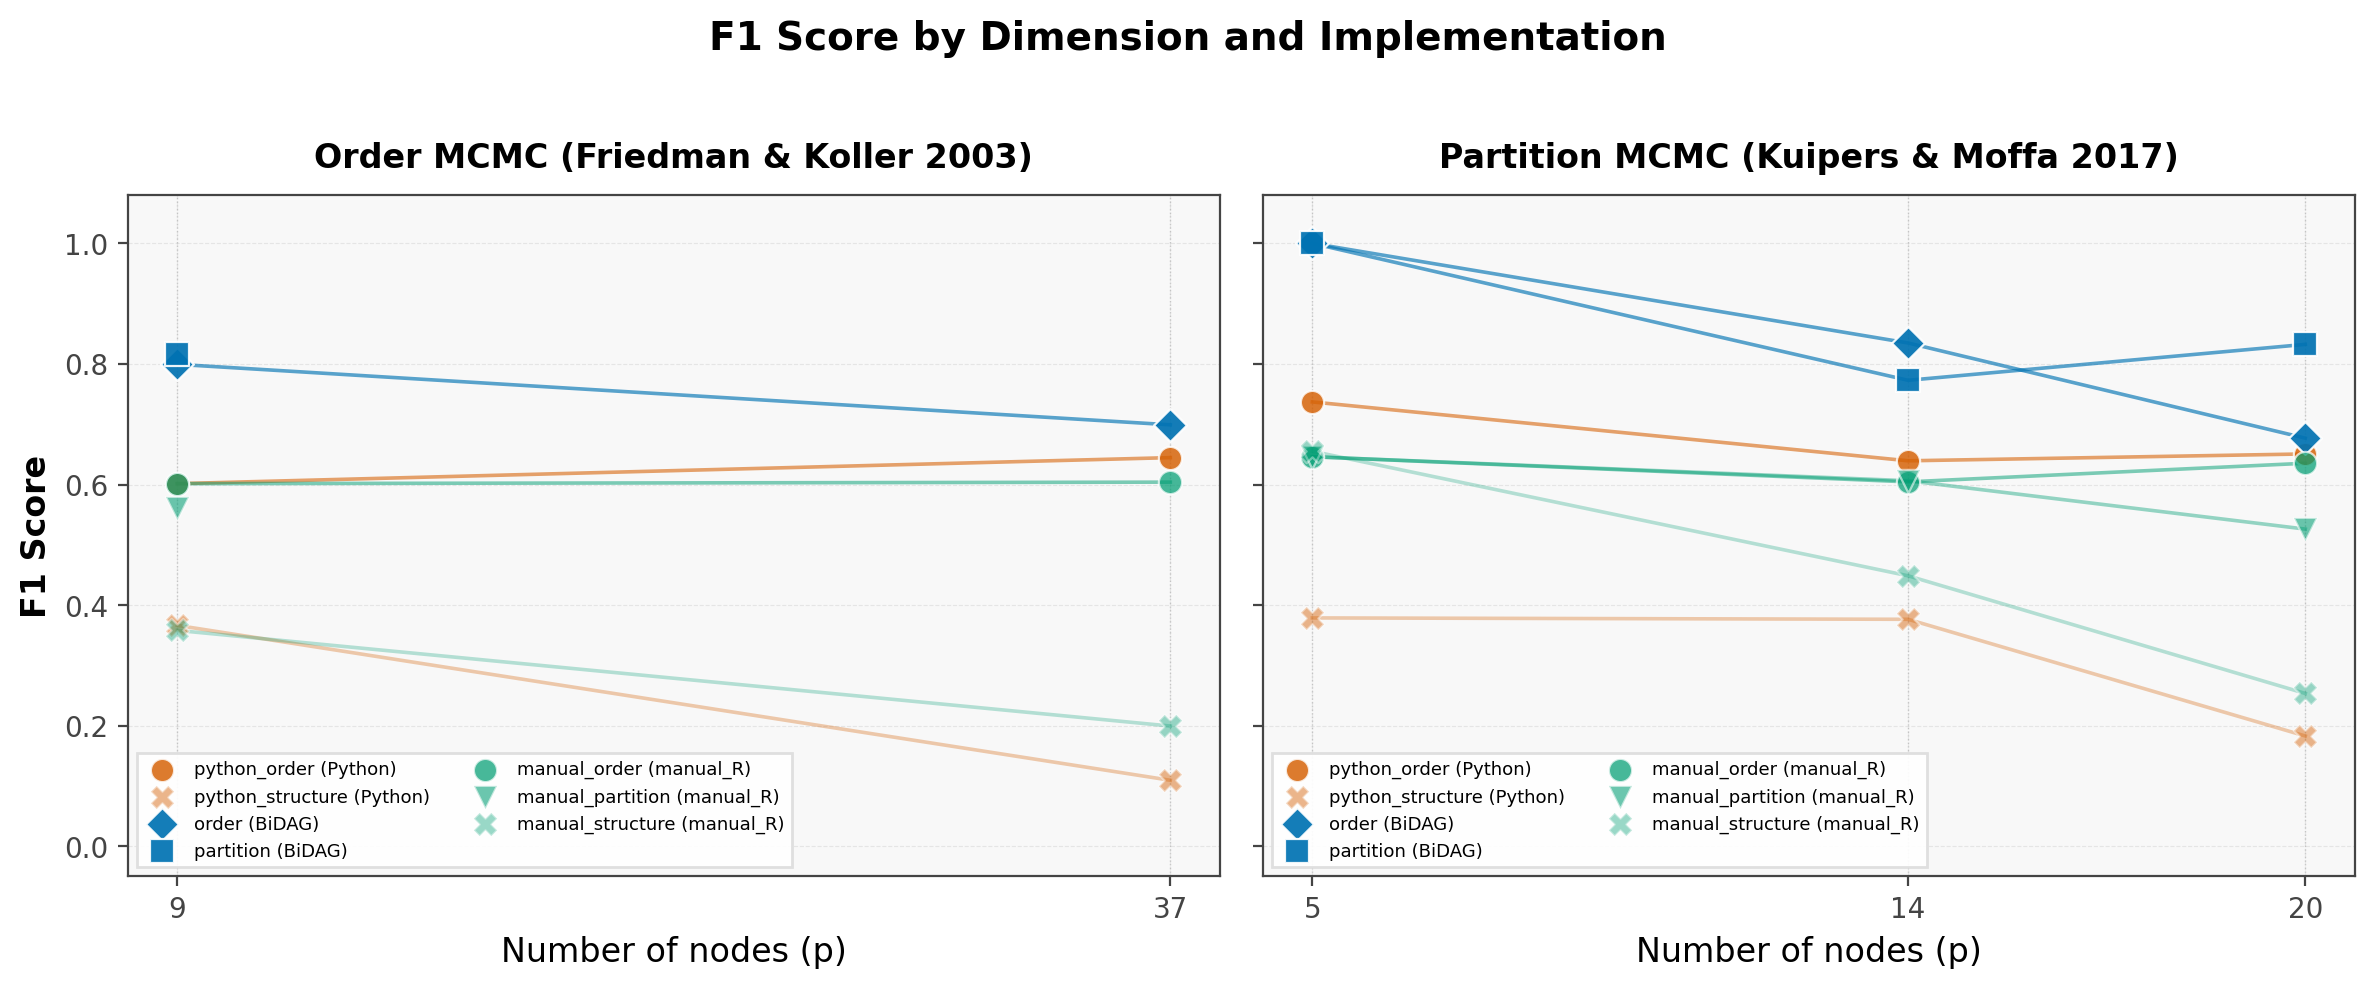
\includegraphics[width=0.92\linewidth]{figures/medium_original_reproduction/medium_f1_shd_compare.png}
\caption{按实验组分面的 F1 散点图：每个点代表一次 MCMC 运行，颜色区分实现方式，形状区分具体方法}
\label{fig:medium_f1_shd}
\end{figure}

图 \ref{fig:medium_f1_shd} 以散点图形式按实验组（Order MCMC / Partition MCMC）分面展示所有成功运行结果。图中显示，BiDAG 在多数设置下位于较高 F1 区域；Python 实现的 order MCMC 与 R 自主 order 在趋势上接近；R 自主 Structure MCMC 在 $p \geq 14$ 后 F1 下降。由于三类实现的评分函数和底层优化并不完全一致，该图主要用于展示趋势和工程差异，而不是进行严格的同源算法性能检验。

\begin{figure}[htbp]
\centering
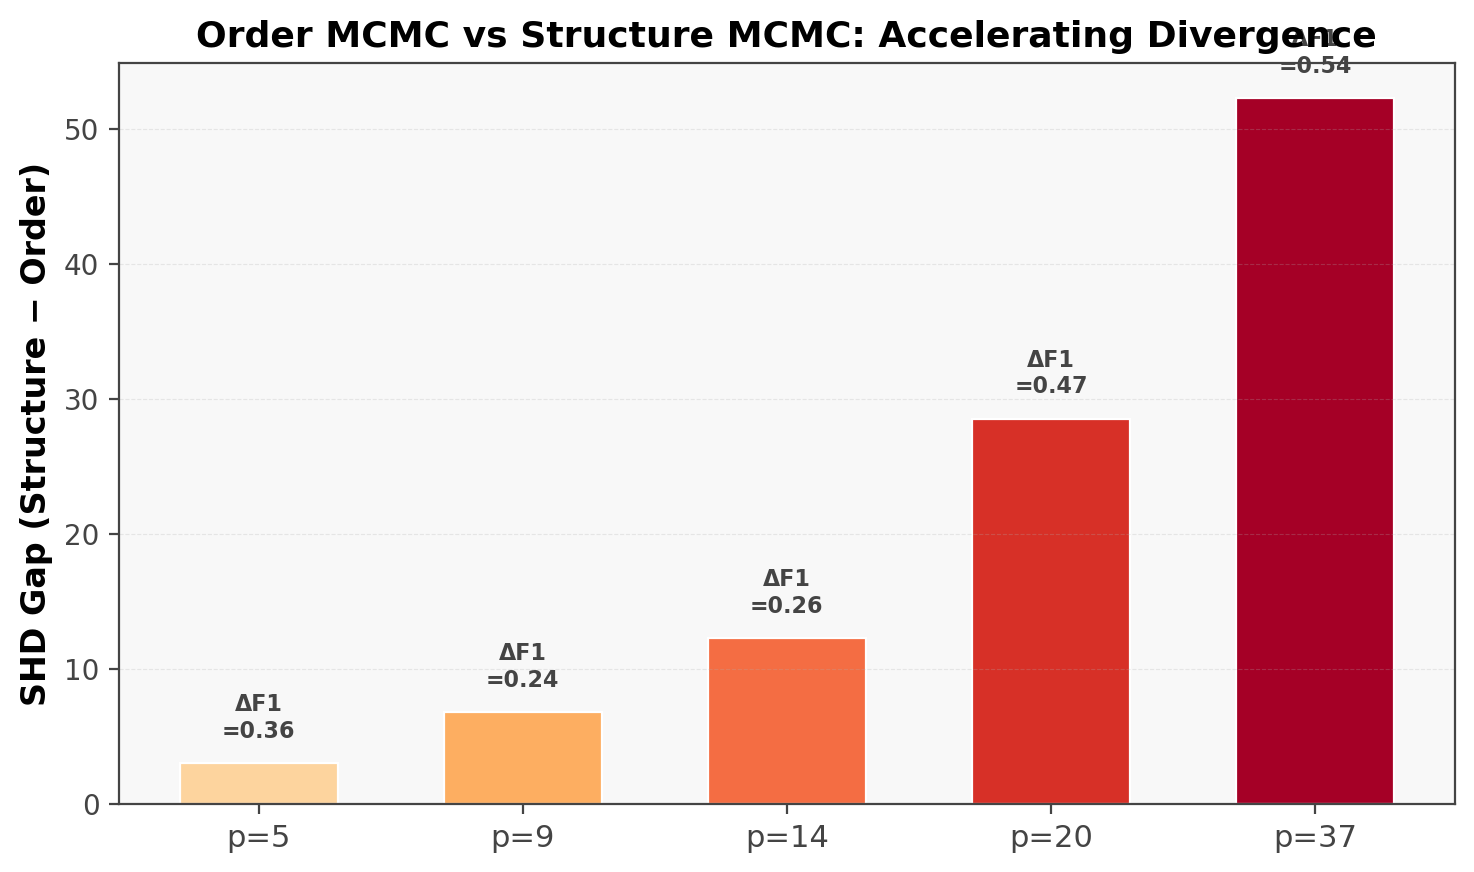
\includegraphics[width=0.92\linewidth]{figures/medium_original_reproduction/order_structure_gap.png}
\caption{Order MCMC 与 Structure MCMC 的 SHD 差距随维度 $p$ 变化（Python 实现）}
\label{fig:order_structure_gap}
\end{figure}

图 \ref{fig:order_structure_gap} 展示了两种方法的 SHD 差距从 $p=5$ 时的 3 个点扩大到 $p=37$ 时的 52 个点，柱顶标注了对应的 F1 差值。

\begin{figure}[htbp]
\centering
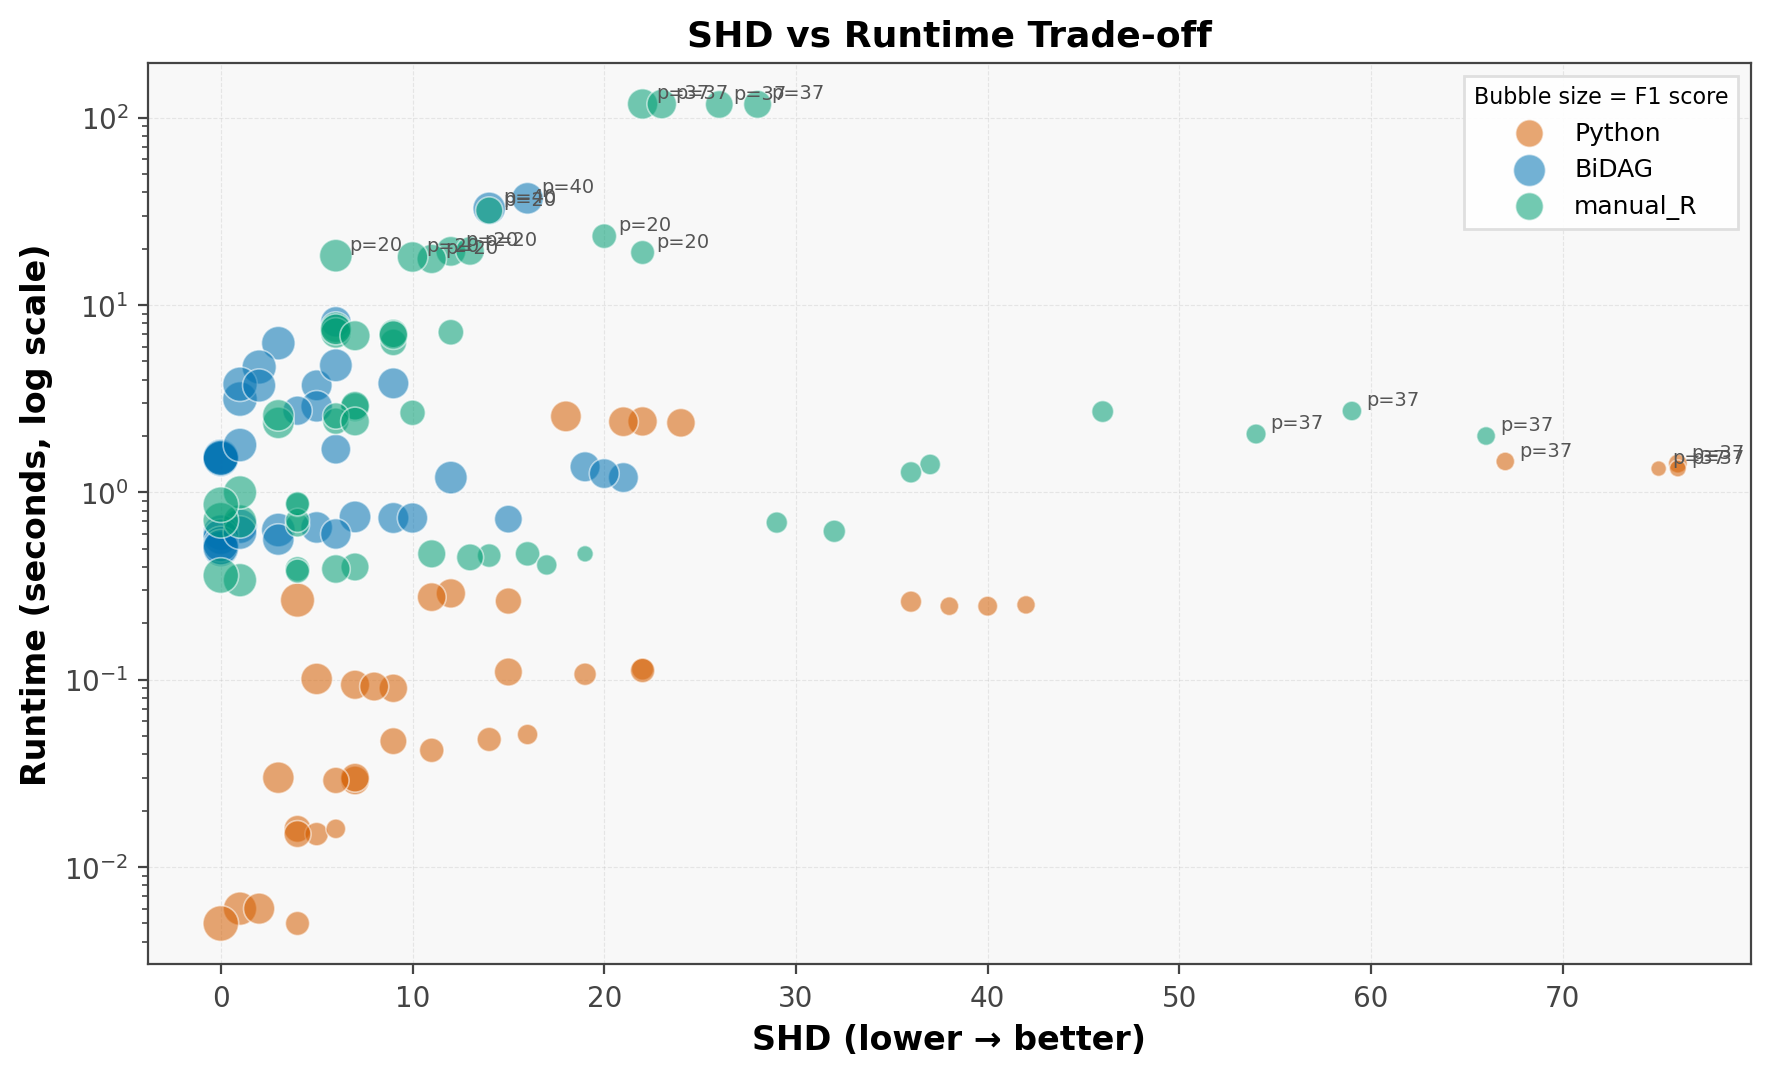
\includegraphics[width=0.88\linewidth]{figures/medium_original_reproduction/medium_runtime_compare.png}
\caption{SHD vs 运行时间的气泡图：气泡大小 = F1，颜色区分实现方式}
\label{fig:medium_runtime}
\end{figure}

图 \ref{fig:medium_runtime} 以对数纵轴展示运行时间对比：Python/numpy 实现和 BiDAG 的运行时间整体低于 R 自主实现，且差距在较大 $p$ 下更清晰。manual\_R 的 structure 方法在 $p \geq 14$ 后出现恢复质量下降，但本组 134 次 MCMC 运行均完成脚本执行。

\begin{table}[htbp]
\centering
\caption{各维度 $p$ 下的最高单次 F1 及三种实现的最高 F1}
\label{tab:impl_compare}
\begin{tabular}{c l c c c c c}
\toprule
$p$ & Best Single Run & SHD & F1 & Python F1 & BiDAG F1 & manual F1 \\
\midrule
5 & python\_order (Py) & 0.0 & 1.000 & 1.000 & 1.000 & 1.000 \\
9 & partition (BD) & 1.0 & 0.923 & 0.750 & 0.923 & 0.750 \\
14 & order (BD) & 0.0 & 1.000 & 0.750 & 1.000 & 0.710 \\
20 & partition (BD) & 2.0 & 0.913 & 0.909 & 0.913 & 0.818 \\
37 & order (BD) & 12.0 & 0.818 & 0.711 & 0.818 & 0.682 \\
\bottomrule
\end{tabular}
\end{table}


表 \ref{tab:impl_compare} 给出了每个维度下最高单次 F1 对应的方法，并同时列出三类实现各自达到的最高 F1。该表用于补充展示不同实现路径的上界表现；由于它基于单次运行最大值，而非均值，解释时应与表 \ref{tab:medium_original_summary} 的平均结果结合。

本实验采用三种实现路径并非为了给出单一排名，而是为了区分算法表示、评分函数和工程实现三类因素。Python 实现和 R 自主实现共享相同的 Gaussian BIC 型评分，因而可用于检查自主实现逻辑在不同语言中的一致趋势；二者的运行时间差异主要反映 numpy 向量化与纯 R 循环之间的工程差异。BiDAG 采用 BGe 边际似然评分和包内搜索空间处理，结果不能与 BIC 评分下的自主实现作完全等价比较，但可作为成熟工程实现的参照。

综合上述结果，该对照实验提供了三点补充观察：第一，在本文模拟设置下，Order MCMC 相比 Structure MCMC 更能维持中等规模下的结构恢复效果；第二，BiDAG partition 在 $p=20$ 设置下优于 BiDAG order，支持 partition 表示在部分设置下缓解排序偏差的作用；第三，Python/numpy、R 自主实现和 BiDAG 三路结果共同说明，结构学习实验中的性能差异同时来自状态空间设计、评分函数选择和底层工程实现。

\newpage
% ======================================================================
\section{讨论}
% ======================================================================

\subsection{状态空间设计}

实验结果表明，MCMC 采样器的效率在很大程度上取决于状态空间的选择。Structure MCMC 的状态与推断目标直接对应，但局部移动能力和无环检查开销限制了其在节点数增加后的表现。Order MCMC 通过将状态重构为排列消除了无环检查，代价是引入了排列偏差。Partition MCMC 进一步使用有序 partition 作为状态表示，在本文的部分实验设置下取得了比 Order MCMC 更高的结构恢复精度。

这一现象提示了一个更具一般性的 MCMC 设计考量：当目标空间本身不利于高效采样时，转向一个更大但结构更规整的辅助空间可能有助于改善混合效率，前提是辅助空间到目标空间的映射偏差可控。

\subsection{规模扩展实验的定位}

在本文的规模扩展实验设置中，普通 MCMC 方法随着节点数增加表现出更清晰的计算压力。Iterative MCMC 在 $p=40$ 下的结果说明，"先筛选、后搜索、再修正"的范式可以作为中等规模以上实验的补充方案。本文的主线仍是状态空间设计与实验对比，更大规模网络设置不作为本文展开重点。

\subsection{不确定性量化}

传统的 SHD 和 F1 指标仅评价 MAP 图的点估计精度。本文的边后验熵分析提供了一个补充视角：即使 MAP 图的结构恢复精度相近，不同方法对结构不确定性的量化结果仍可能存在差异。在科学应用中，了解哪些边的估计较为可靠、哪些仍存在较大不确定性，有时比获得单一最优图更有参考价值。

\subsection{局限与展望}

本文工作存在以下局限：

第一，自主实现采用 Gaussian BIC 型评分，不等价于 BiDAG 中的 BGe/BDeu 边际似然评分。因此，二者的数值差异同时反映了评分函数、父集约束和实现优化的综合影响，不应被解释为单一 MCMC 状态空间设计的优劣。

第二，链长相对较短（1200--3000 步），未进行严格的收敛诊断（如 Gelman-Rubin $\hat{R}$ 统计量）。这主要是因为多方法、多参数组合下的单链运行时间和计算资源限制。第 4.3 节提出的多链诊断框架为未来工作提供了实现蓝图。

第三，本文主要关注模拟数据上的方法比较，尚未将更大规模网络作为主线实验对象。后续若扩展到服务器环境或更长链设置，可进一步检验 iterative 策略在更复杂网络中的表现。

第四，benchmark 网络（Asia、Sachs、ALARM）的实验尚未纳入主线结果。这些标准网络提供了与文献中的其他方法进行交叉比较的桥梁，是未来扩展的重要方向。

\FloatBarrier
\newpage
% ======================================================================
\section{结论}
% ======================================================================

本文围绕贝叶斯网络结构学习中的 MCMC 方法，从算法设计动机出发，比较了 Structure MCMC、Order MCMC、Partition MCMC 和 hybrid/iterative MCMC 四种策略。主要结论如下：

\begin{enumerate}
  \item 状态空间的选择对 MCMC 采样效率有重要影响。Order MCMC 将状态从 DAG 重构为排列以消除无环检查，但引入了排列偏差；Partition MCMC 在本文的部分实验设置下获得了较好的结构恢复精度，并在部分中等规模设置中表现出较低的边后验熵。
  \item 在节点数增加的补充实验中，hybrid/iterative 策略通过条件独立筛选缩小候选边集，为中等规模以上网络提供了一种实用的搜索空间压缩思路。该结论仅基于本文的模拟设置，在其他场景下的表现尚需进一步检验。
  \item 边后验熵和真假边后验分离度为结构不确定性提供了超越 SHD 和 F1 的量化维度。
  \item 自主 MCMC 实现完整呈现了评分计算、proposal 生成、MH 判定和边后验累积的内部过程，为不同状态空间设计提供了可审计的对照；BiDAG 复现实验则体现了成熟包实现中评分函数、父集搜索和底层优化带来的综合优势。
\end{enumerate}

后续工作可从以下方向展开：(1) 在自主采样器中引入 BGe 评分以减少评分函数差异；(2) 引入更长链和多链收敛诊断；(3) 补充 Asia、Sachs 等 benchmark 网络实验；(4) 增加可视化工具用于呈现边后验概率和结构不确定性。

\clearpage
\bibliographystyle{plainnat}
\bibliography{references}

\FloatBarrier
\newpage
\appendix

\section{实验环境与可复现性}

\subsection{软件环境}

本文主线实验基于 R 语言（版本 4.5.1）完成；第 6.10 节的中等规模关键论文趋势对照实验另包含 Python/numpy 实现，用于与 R 自主实现进行交叉验证。核心依赖包括：\texttt{BiDAG}（贝叶斯网络结构学习的 MCMC 采样与评分）\citep{suter2023bidag}、\texttt{igraph}（有向图操作与 DAG 判定）、\texttt{ggplot2}（实验结果可视化）以及 \texttt{dplyr}（数据处理）。环境通过 \texttt{renv} 实现依赖版本管理：执行 \texttt{source("restore\_environment.R")} 即可根据 \texttt{renv.lock} 安装所需包的锁定版本，确保实验的可复现性。

\subsection{代码结构}

项目代码分为三个层次。核心函数层（\texttt{R/}）包含自主 MCMC 采样器的完整实现（\texttt{manual\_mcmc.R}，约 420 行）、BiDAG 调用封装（\texttt{bidag\_runner.R}）、数据模拟（\texttt{simulation.R}）、评价指标（\texttt{metrics.R}）和可视化（\texttt{plotting.R}）。实验入口层（\texttt{scripts/}）包含九个独立实验脚本，分别覆盖初步运行检查、自主实现验证、低维比较、中等规模比较、iterative 补充实验、样本量影响、父集约束敏感性、边后验不确定性分析和收敛诊断等实验。报告生成层（\texttt{report/}）包含 LaTeX 源文件、参考文献和自动生成的图表。源代码仓库已整理至 GitHub：\url{https://github.com/Eurekaimer/statcomp-project}，其中包含复现实验所需的代码、notebook、模拟数据和结果文件。

\subsection{实验复现}

完整实验复现步骤如下：

\begin{enumerate}[label=(\arabic*)]
  \item \textbf{环境准备。} 在 RStudio 中打开 \texttt{Project/} 目录，依次执行：
  \begin{verbatim}
  install.packages("renv")
  source("restore_environment.R")
  source("R/load_project.R")
  load_project()
  \end{verbatim}
  其中 \texttt{restore\_environment.R} 调用 \texttt{renv::restore()} 根据 \texttt{renv.lock} 安装所有依赖包的精确版本。

  \item \textbf{初步运行检查。} 执行 \texttt{source("scripts/smoke\_test.R")}，验证环境和主链路正常。

  \item \textbf{主线实验。} 执行 \texttt{source("run\_all.R")} 依次运行全部主线实验（自主实现验证、低维/中等规模比较、iterative 补充实验、样本量影响等）。各实验脚本以独立子进程运行，单个实验失败不影响后续实验。

  \item \textbf{报告生成。} 执行 \texttt{source("scripts/build\_report\_assets.R")} 将图表整理至报告目录，随后编译 LaTeX 源文件生成 PDF。
\end{enumerate}

实验输出文件的对应关系如下：
\begin{itemize}
  \item 表格输出以 CSV 格式保存于 \texttt{results/tables/}；
  \item 报告图像保存于 \texttt{results/figures/}；
  \item 报告中的主要数值和图像可由上述结果文件及作图脚本对应核对。
\end{itemize}

\end{document}
